
\documentclass{sig-alternate}
\usepackage{polski}
\usepackage[utf8]{inputenc}
\usepackage{graphicx}
\usepackage{rotating}
\usepackage[dvipsnames]{xcolor}  % color is sufficient
\pdfpagewidth=8.5in
\pdfpageheight=11in
\special{papersize=8.5in,11in}

    \renewcommand{\topfraction}{1}	% max fraction of floats at top
    \renewcommand{\bottomfraction}{1} % max fraction of floats at bottom
    %   Parameters for TEXT pages (not float pages):
    \setcounter{topnumber}{3}
    \setcounter{bottomnumber}{3}
    \setcounter{totalnumber}{3}     % 2 may work better
    \setcounter{dbltopnumber}{4}    % for 2-column pages
    \renewcommand{\dbltopfraction}{1}	% fit big float above 2-col. text
    \renewcommand{\textfraction}{0.0}	% allow minimal text w. figs
    %   Parameters for FLOAT pages (not text pages):
    \renewcommand{\floatpagefraction}{0.80}	% require fuller float pages
	% N.B.: floatpagefraction MUST be less than topfraction !!
    \renewcommand{\dblfloatpagefraction}{0.7}	% require fuller float pages

%%%%%%%%%%%%%%%%%%%%%%   END OF PREAMBLE   %%%%%%%%%%%%%%%%%%%%%%%%%%%%%%%%%%%%

%%%%%%%%%%%%%%%%%%%%%%%%%%%%%%%%%%%%%%%%%%%%%%%%%%%%%%%%%%%%%%%%%%%%%%%%%%%%%%%
%%%%%%%%% TO BE EDITED %%%%%%%%%%%%%%%%%%%%%%%%%%%%%%%%%%%%%%%%%%%%%%%%%%%%%%%%
%%%%%%%%%%%%%%%%%%%%%%%%%%%%%%%%%%%%%%%%%%%%%%%%%%%%%%%%%%%%%%%%%%%%%%%%%%%%%%%
% rungeneric.py writes data into a subfolder of ppdata
\newcommand{\bbobdatapath}{ppdata/} % default output folder of rungeneric.py
\input{\bbobdatapath bbob_pproc_commands.tex} % provide default of algname and algfolder
% \renewcommand{\algname}{MYNAME}  % name of algorithm as it should appear in the text
% \renewcommand{\algfolder}{ABC/} % subfolder of \bbobdatapath for processed algorithm
%%%%%%%%%%%%%%%%%%%%%%%%%%%%%%%%%%%%%%%%%%%%%%%%%%%%%%%%%%%%%%%%%%%%%%%%%%%%%%%
%%%%%%%%%%%%%%%%%%%%%%%%%%%%%%%%%%%%%%%%%%%%%%%%%%%%%%%%%%%%%%%%%%%%%%%%%%%%%%%
%%%%%%%%%%%%%%%%%%%%%%%%%%%%%%%%%%%%%%%%%%%%%%%%%%%%%%%%%%%%%%%%%%%%%%%%%%%%%%%
\graphicspath{{\bbobdatapath\algfolder}}

\newcommand{\DIM}{\ensuremath{\mathrm{DIM}}}
\newcommand{\ERT}{\ensuremath{\mathrm{ERT}}}
\newcommand{\FEvals}{\ensuremath{\mathrm{FEvals}}}
\newcommand{\nruns}{\ensuremath{\mathrm{Nruns}}}
\newcommand{\Dfb}{\ensuremath{\Delta f_{\mathrm{best}}}}
\newcommand{\Df}{\ensuremath{\Delta f}}
\newcommand{\nbFEs}{\ensuremath{\mathrm{\#FEs}}}
\newcommand{\fopt}{\ensuremath{f_\mathrm{opt}}}
\newcommand{\ftarget}{\ensuremath{f_\mathrm{t}}}
\newcommand{\CrE}{\ensuremath{\mathrm{CrE}}}
\newcommand{\change}[1]{{\color{red} #1}}

\begin{document}
%
% --- Author Metadata here ---
%\conferenceinfo{GECCO'13,} {July 6-10, 2013, Amsterdam, The Netherlands.}
%\CopyrightYear{2013}
%\crdata{TBA}
%\clubpenalty=10000
%\widowpenalty = 10000
% --- End of Author Metadata ---

\title{Modyfikacje/hybrydyzacje algorytmu PSO w zadaniu optymalizacji globalnej wielowymiarowej funkcji ciągłej
% \titlenote{If needed}
}
\subtitle{PSO-DE Hybrid
%\titlenote{Submission deadline: March 28th.}}
%Camera-ready paper due April 17th.}}
}
%
% You need the command \numberofauthors to handle the 'placement
% and alignment' of the authors beneath the title.
%
% For aesthetic reasons, we recommend 'three authors at a time'
% i.e. three 'name/affiliation blocks' be placed beneath the title.
%
% NOTE: You are NOT restricted in how many 'rows' of
% "name/affiliations" may appear. We just ask that you restrict
% the number of 'columns' to three.
%
% Because of the available 'opening page real-estate'
% we ask you to refrain from putting more than six authors
% (two rows with three columns) beneath the article title.
% More than six makes the first-page appear very cluttered indeed.
%
% Use the \alignauthor commands to handle the names
% and affiliations for an 'aesthetic maximum' of six authors.
% Add names, affiliations, addresses for
% the seventh etc. author(s) as the argument for the
% \additionalauthors command.
% These 'additional authors' will be output/set for you
% without further effort on your part as the last section in
% the body of your article BEFORE References or any Appendices.

\numberofauthors{1} %  in this sample file, there are a *total*
% of EIGHT authors. SIX appear on the 'first-page' (for formatting
% reasons) and the remaining two appear in the \additionalauthors section.
%
\author{
% You can go ahead and credit any number of authors here,
% e.g. one 'row of three' or two rows (consisting of one row of three
% and a second row of one, two or three).
%
% The command \alignauthor (no curly braces needed) should
% precede each author name, affiliation/snail-mail address and
% e-mail address. Additionally, tag each line of
% affiliation/address with \affaddr, and tag the
% e-mail address with \email.
%
% 1st. author
\alignauthor
Jakub Ruszkowski, Mateusz Kaczmarski\\ %\titlenote{Dr.~Trovato insisted his name be first.}\\
       \affaddr{Politechnika Warszawska}\\
		\affaddr{Wydział Matematyki i Nauk Informacyjnych}\\
%% 2nd. author
%\alignauthor
%G.K.M. Tobin\titlenote{The secretary disavows
%any knowledge of this author's actions.}\\
%       \affaddr{Institute for Clarity in Documentation}\\
%       \affaddr{P.O. Box 1212}\\
%       \affaddr{Dublin, Ohio 43017-6221}\\
%       \email{webmaster@marysville-ohio.com}
} % author


\maketitle
\begin{abstract}
Dokumentacja uzyskanych wyników hybrydy PSO-DE
\end{abstract}

% Add any ACM category that you feel is needed
\category{G.1.6}{Numerical Analysis}{Optimization}[global optimization,
unconstrained optimization]
\category{F.2.1}{Analysis of Algorithms and Problem Complexity}{Numerical Algorithms and Problems}

% Complete with anything that is needed
\terms{Algorithms}

% Complete with anything that is needed
\keywords{Benchmarking, PSODE, Optymalizacja wielowymiarowej funkcji ciaglej}

% \section{Introduction}
%
% \section{Algorithm Presentation}
%
% \section{Experimental Procedure}
%
%%%%%%%%%%%%%%%%%%%%%%%%%%%%%%%%%%%%%%%%%%%%%%%%%%%%%%%%%%%%%%%%%%%%%%%%%%%%%%%
\section{CPU Timing}
%%%%%%%%%%%%%%%%%%%%%%%%%%%%%%%%%%%%%%%%%%%%%%%%%%%%%%%%%%%%%%%%%%%%%%%%%%%%%%%
% note that the following text is just a proposal and can/should be changed to your needs:
In order to evaluate the CPU timing of the algorithm, we have run the {PSO-DE Hybrid} on the function $f_{8}$ with restarts for at least 30 seconds and until a maximum budget equal to {$400 (D + 2)$} is reached. The code was run on a {Windows 8 Intel(R) Core(TM) i7-4500U CPU @ 2.39GHz} with {1} processor and {2} cores. The time per function evaluation for dimensions 2, 3, 5, 10, 20 equals $1,9e^{-10}$, $2,2e^{-10}$, $2,4e^{-10}$, $3,5e^{-10}$ and $6,1e^{-10}$ seconds respectively. 


%%%%%%%%%%%%%%%%%%%%%%%%%%%%%%%%%%%%%%%%%%%%%%%%%%%%%%%%%%%%%%%%%%%%%%%%%%%%%%%
\section{Results}
%%%%%%%%%%%%%%%%%%%%%%%%%%%%%%%%%%%%%%%%%%%%%%%%%%%%%%%%%%%%%%%%%%%%%%%%%%%%%%%

Results of \algname\ from experiments according to \cite{hansen2012exp} on the benchmark
functions given in \cite{wp200901_2010,hansen2012fun} are presented in
Figures~\ref{fig:ERTgraphs}, \ref{fig:RLDs}, \ref{tab:ERTloss}, and \ref{fig:ERTlogloss} and in
Tables~\ref{tab:ERTs}.

%%%%%%%%%%%%%%%%%%%%%%%%%%%%%%%%%%%%%%%%%%%%%%%%%%%%%%%%%%%%%%%%%%%%%%%%%%%%%%%
%%%%%%%%%%%%%%%%%%%%%%%%%%%%%%%%%%%%%%%%%%%%%%%%%%%%%%%%%%%%%%%%%%%%%%%%%%%%%%%

% Scaling of ERT with dimension

%%%%%%%%%%%%%%%%%%%%%%%%%%%%%%%%%%%%%%%%%%%%%%%%%%%%%%%%%%%%%%%%%%%%%%%%%%%%%%%
\begin{figure*}
\begin{tabular}{l@{\hspace*{-0.025\textwidth}}l@{\hspace*{-0.025\textwidth}}l@{\hspace*{-0.025\textwidth}}l}
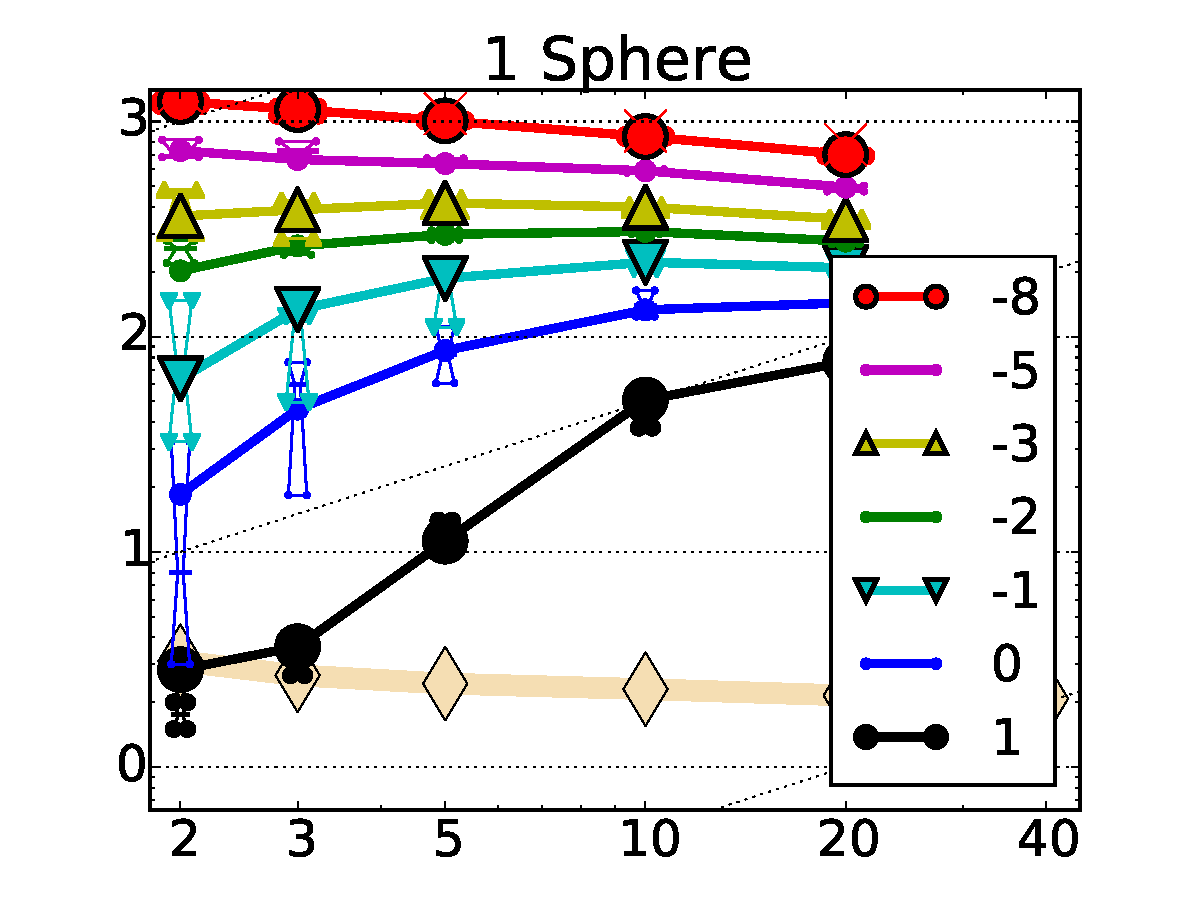
\includegraphics[width=0.268\textwidth]{ppfigdim_f001}&
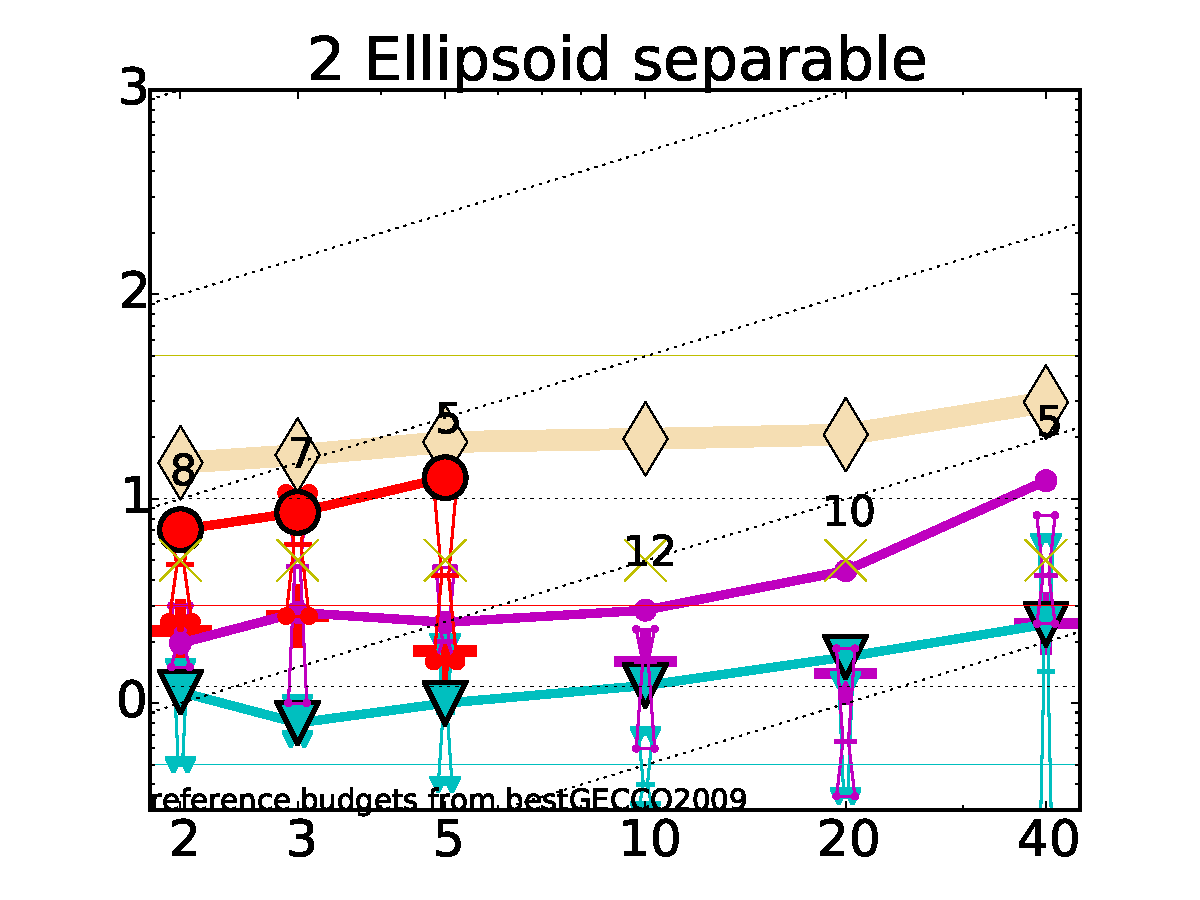
\includegraphics[width=0.268\textwidth]{ppfigdim_f002}&
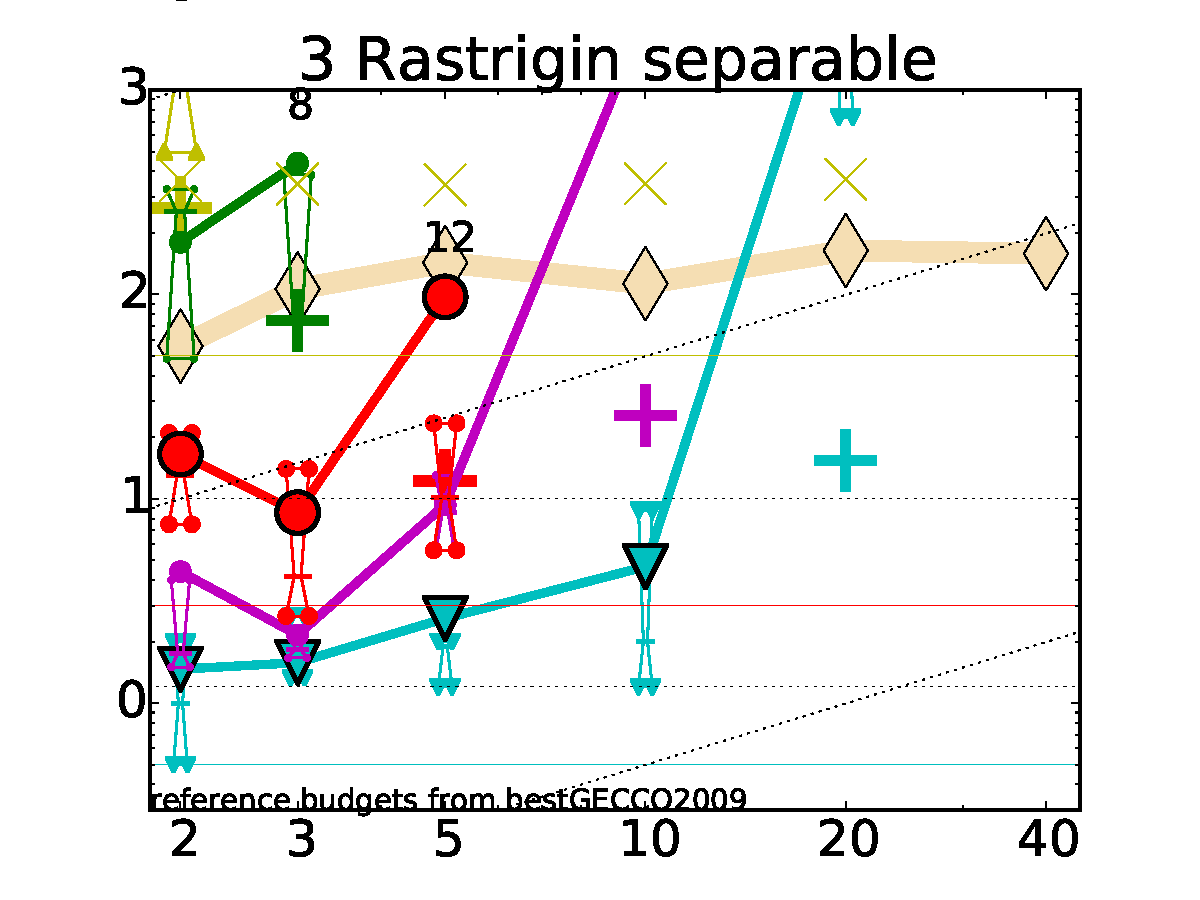
\includegraphics[width=0.268\textwidth]{ppfigdim_f003}&
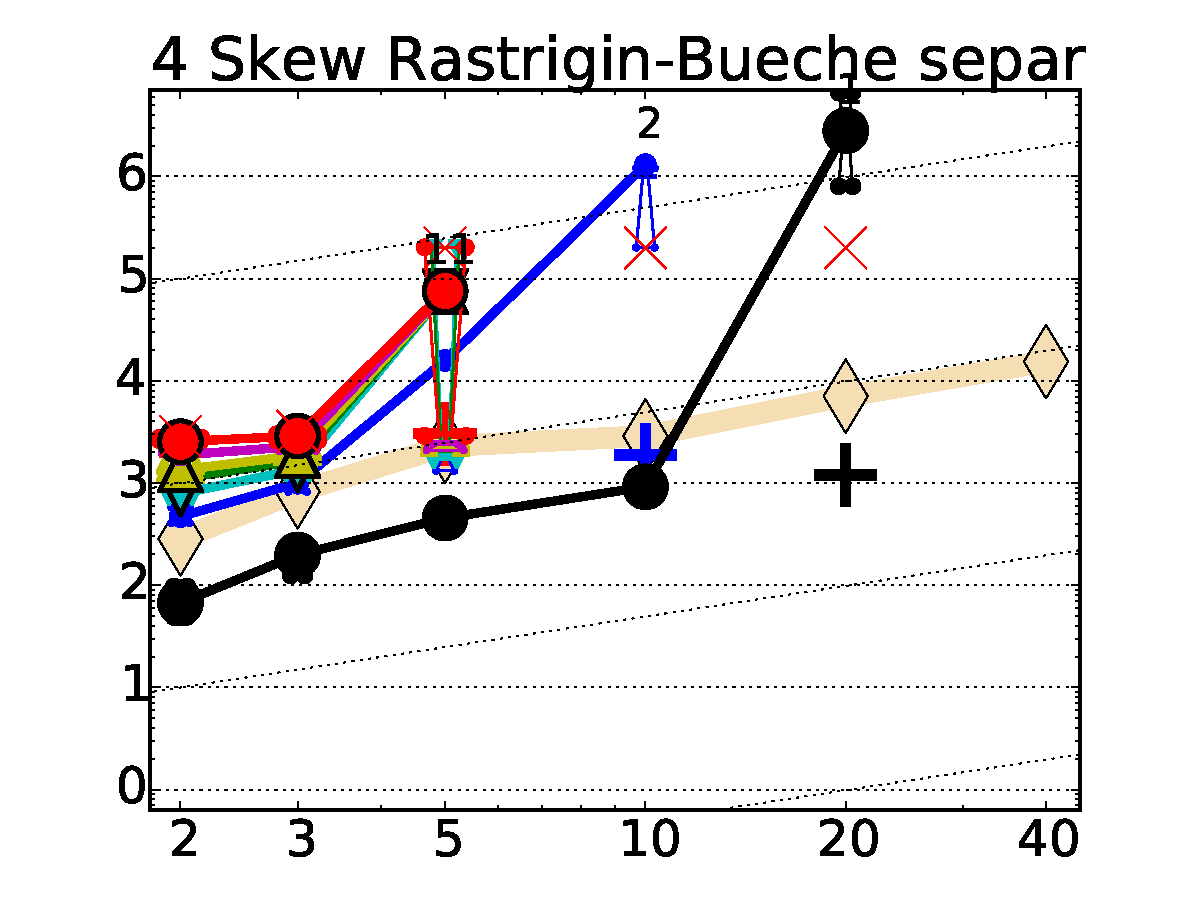
\includegraphics[width=0.268\textwidth]{ppfigdim_f004}\\[-2.2ex]
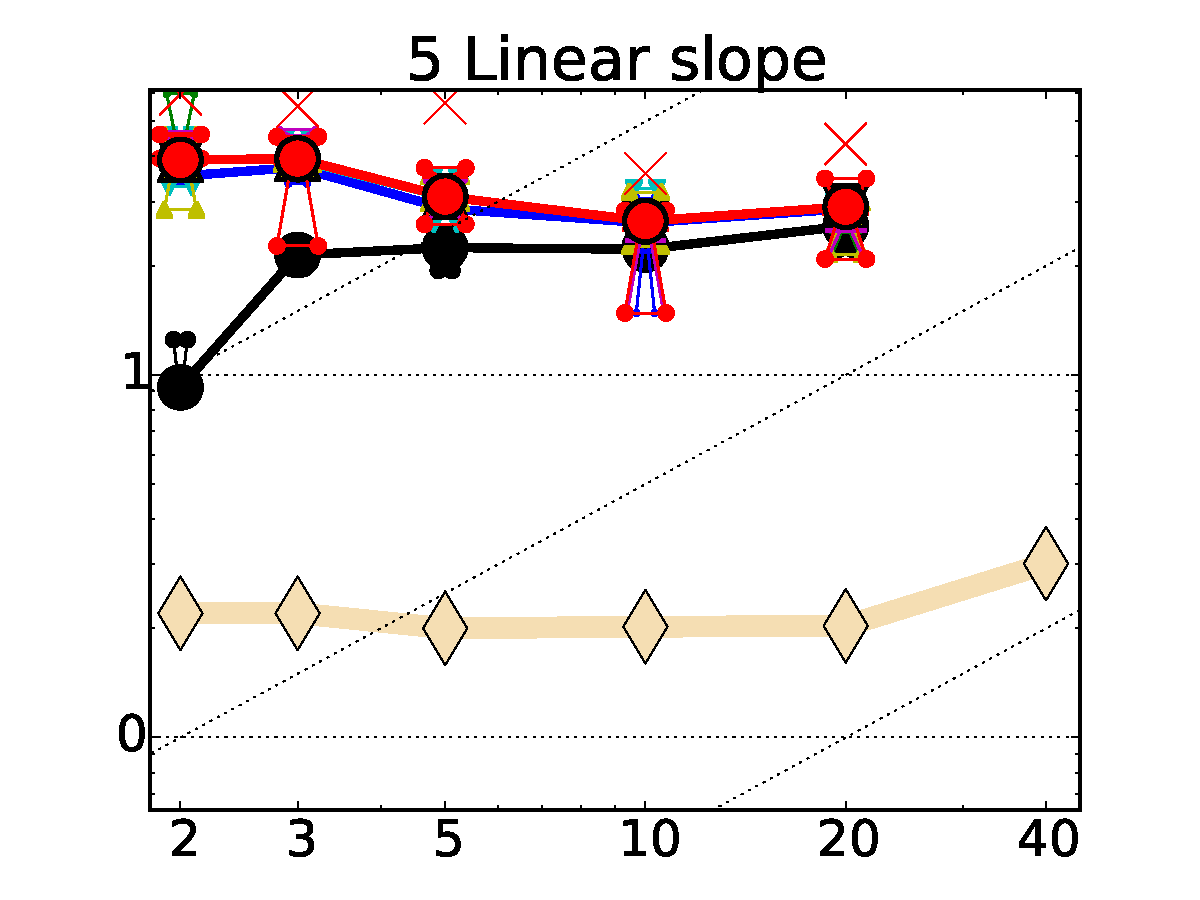
\includegraphics[width=0.268\textwidth]{ppfigdim_f005}&
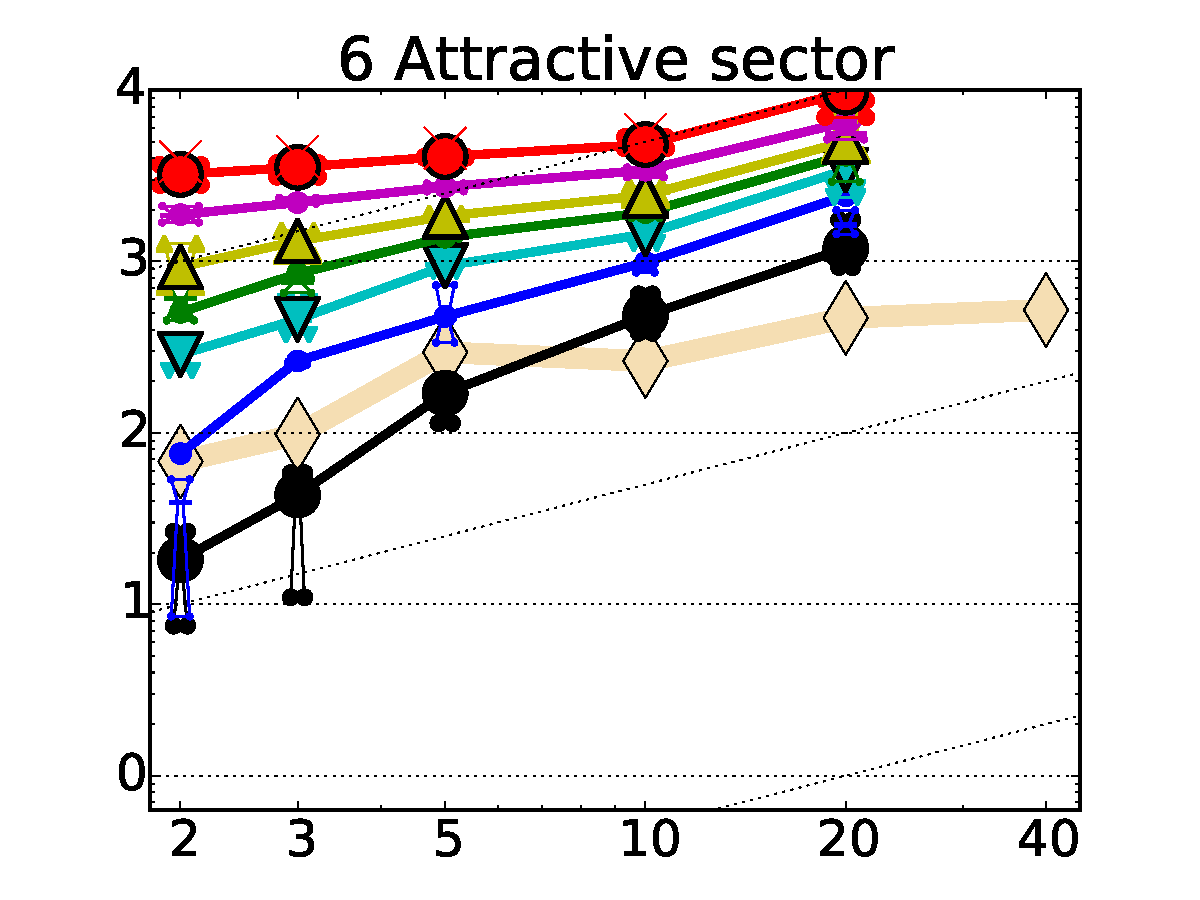
\includegraphics[width=0.268\textwidth]{ppfigdim_f006}&
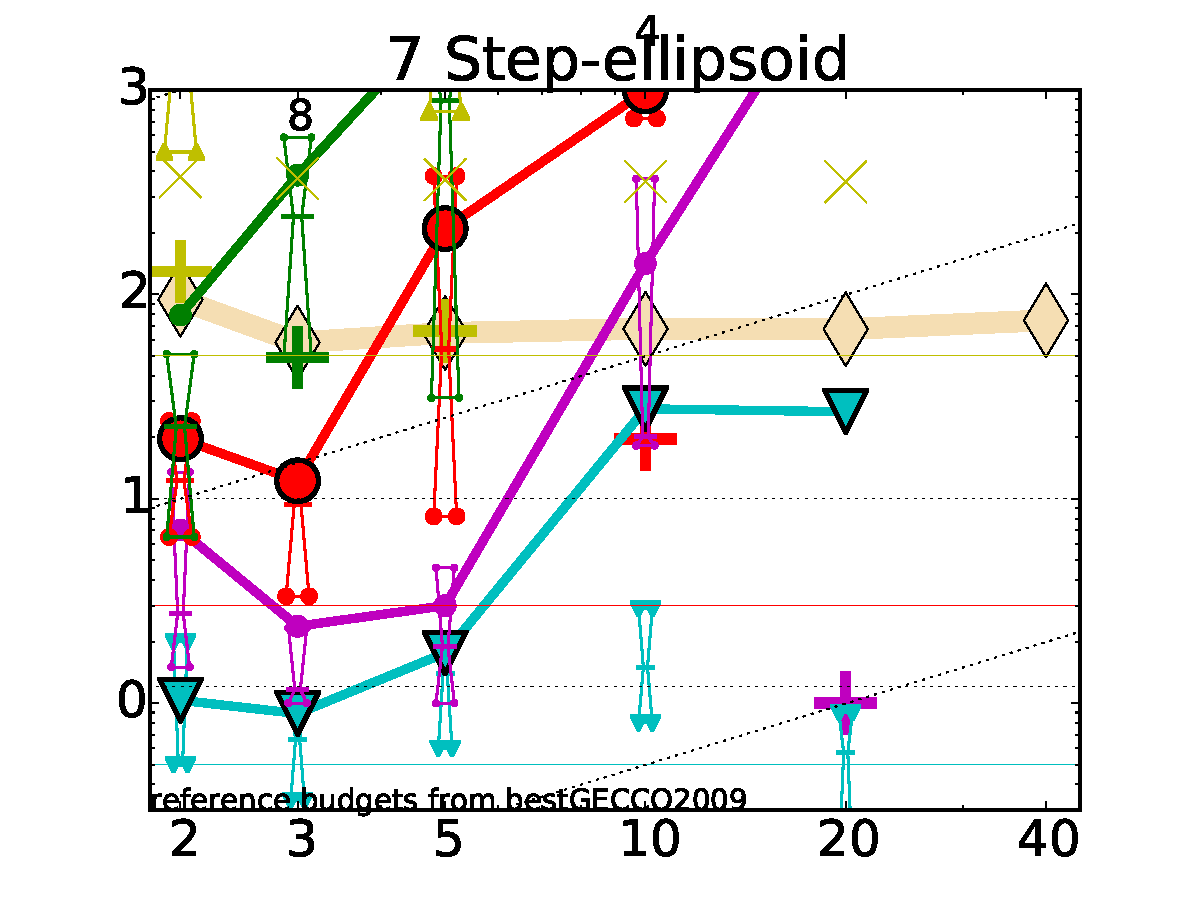
\includegraphics[width=0.268\textwidth]{ppfigdim_f007}&
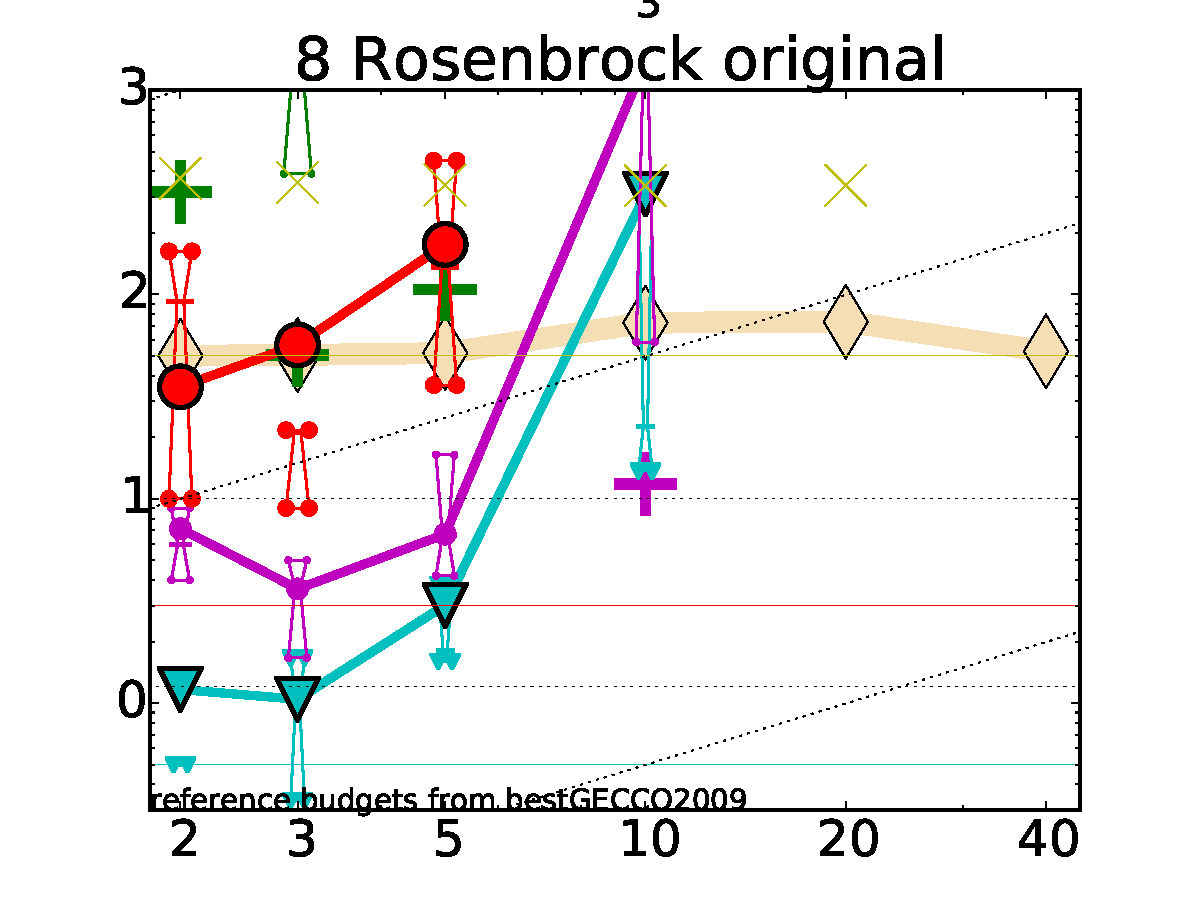
\includegraphics[width=0.268\textwidth]{ppfigdim_f008}\\[-2.2ex]
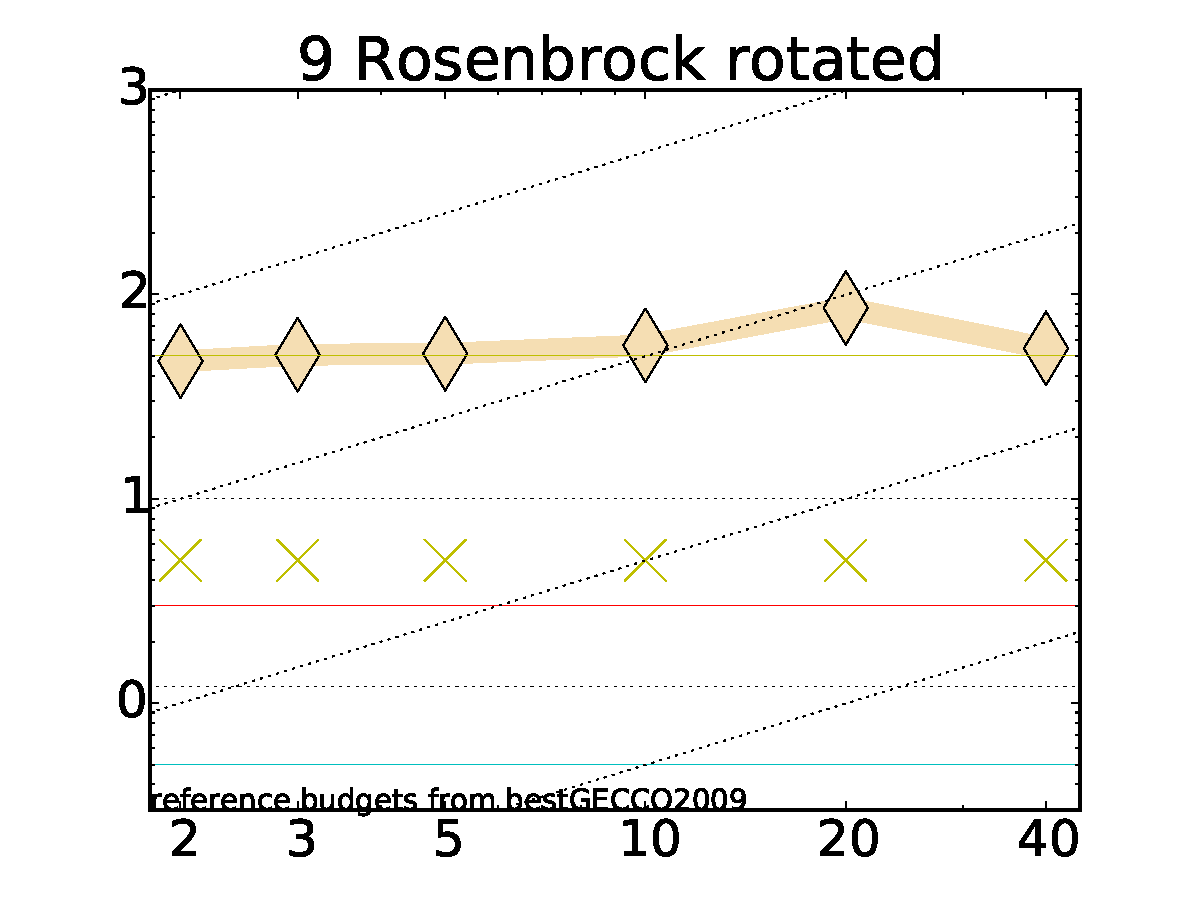
\includegraphics[width=0.268\textwidth]{ppfigdim_f009}&
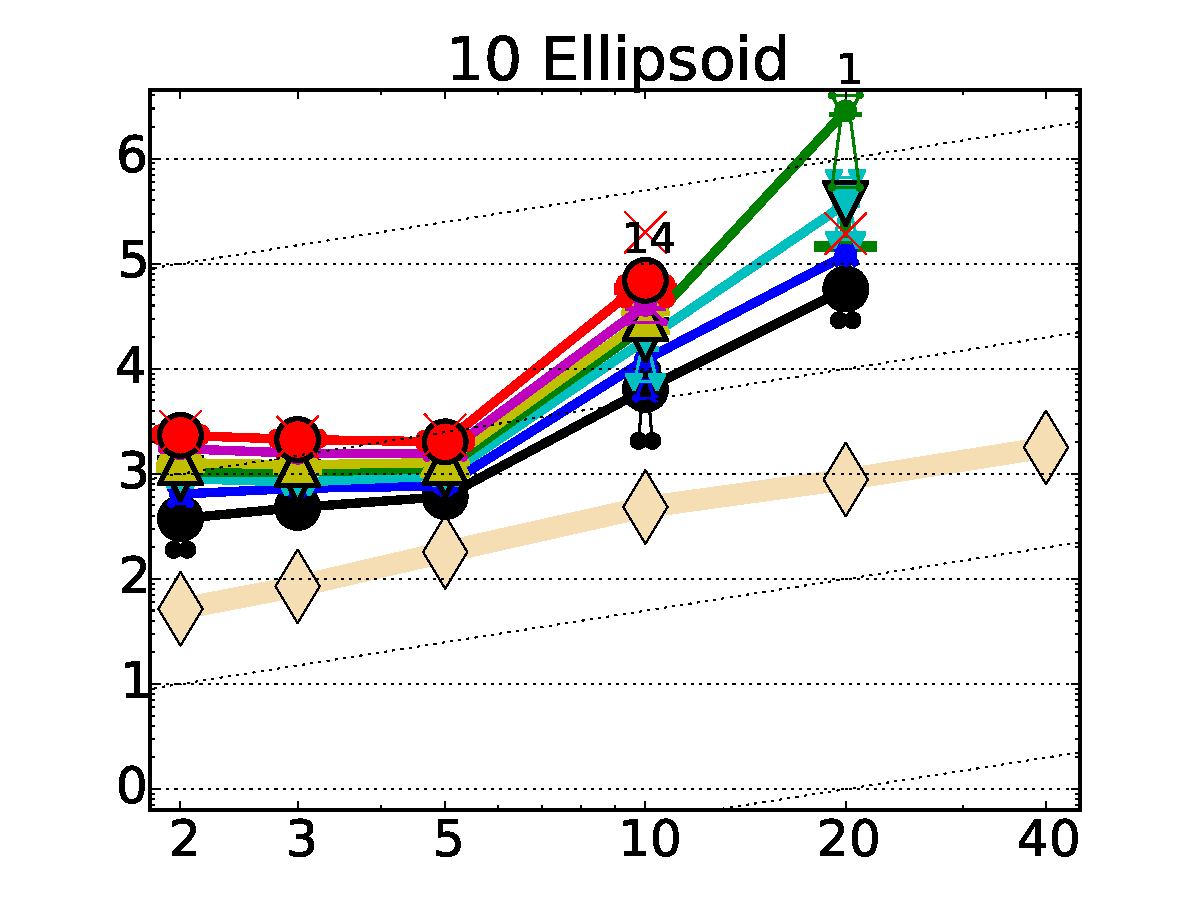
\includegraphics[width=0.268\textwidth]{ppfigdim_f010}&
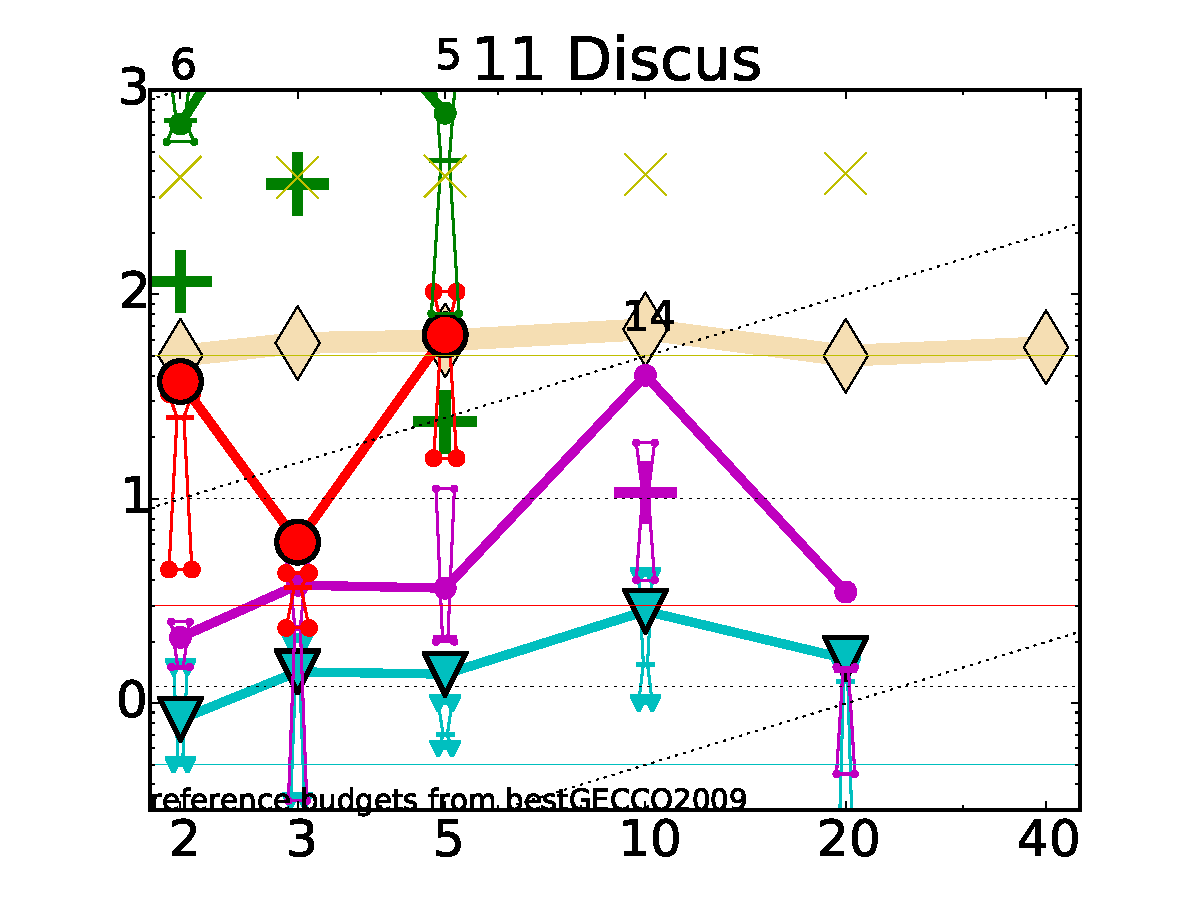
\includegraphics[width=0.268\textwidth]{ppfigdim_f011}&
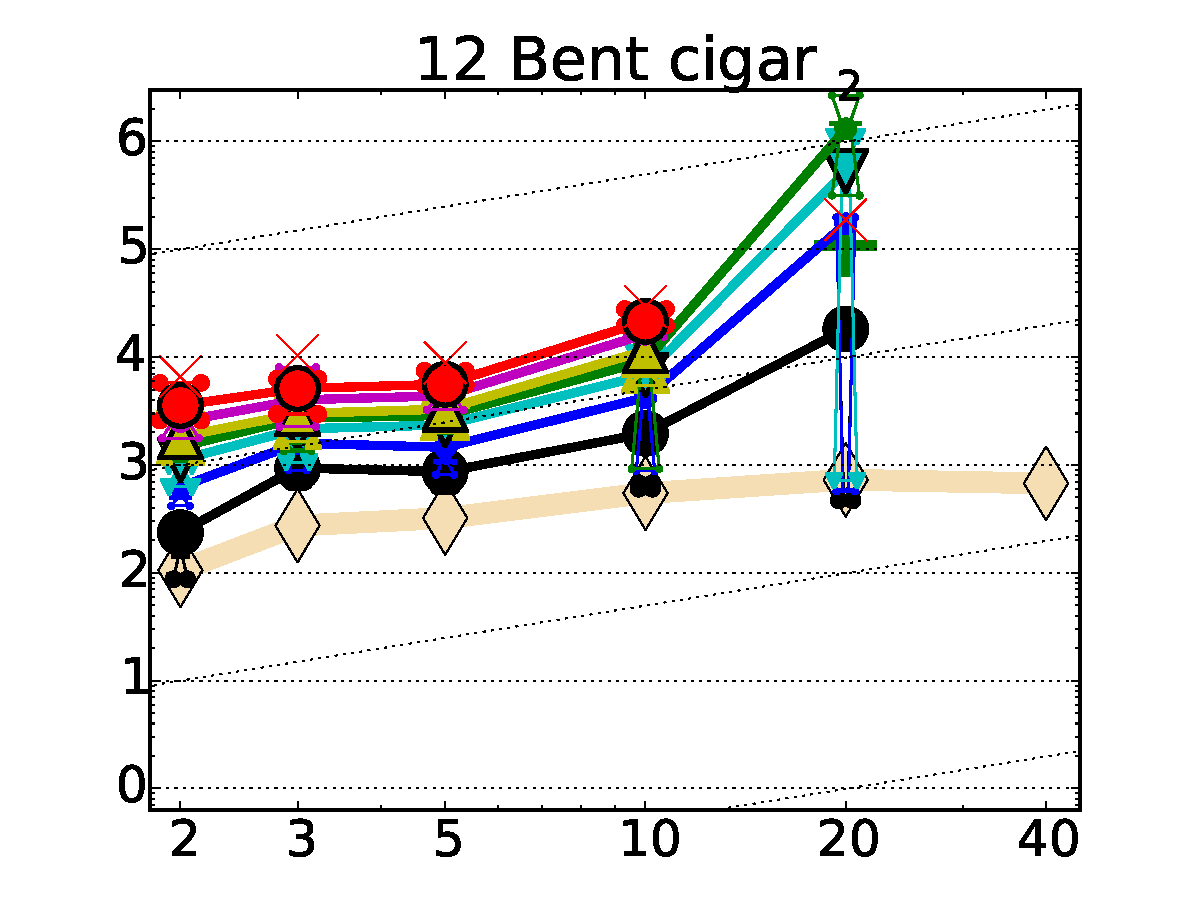
\includegraphics[width=0.268\textwidth]{ppfigdim_f012}\\[-2.2ex]
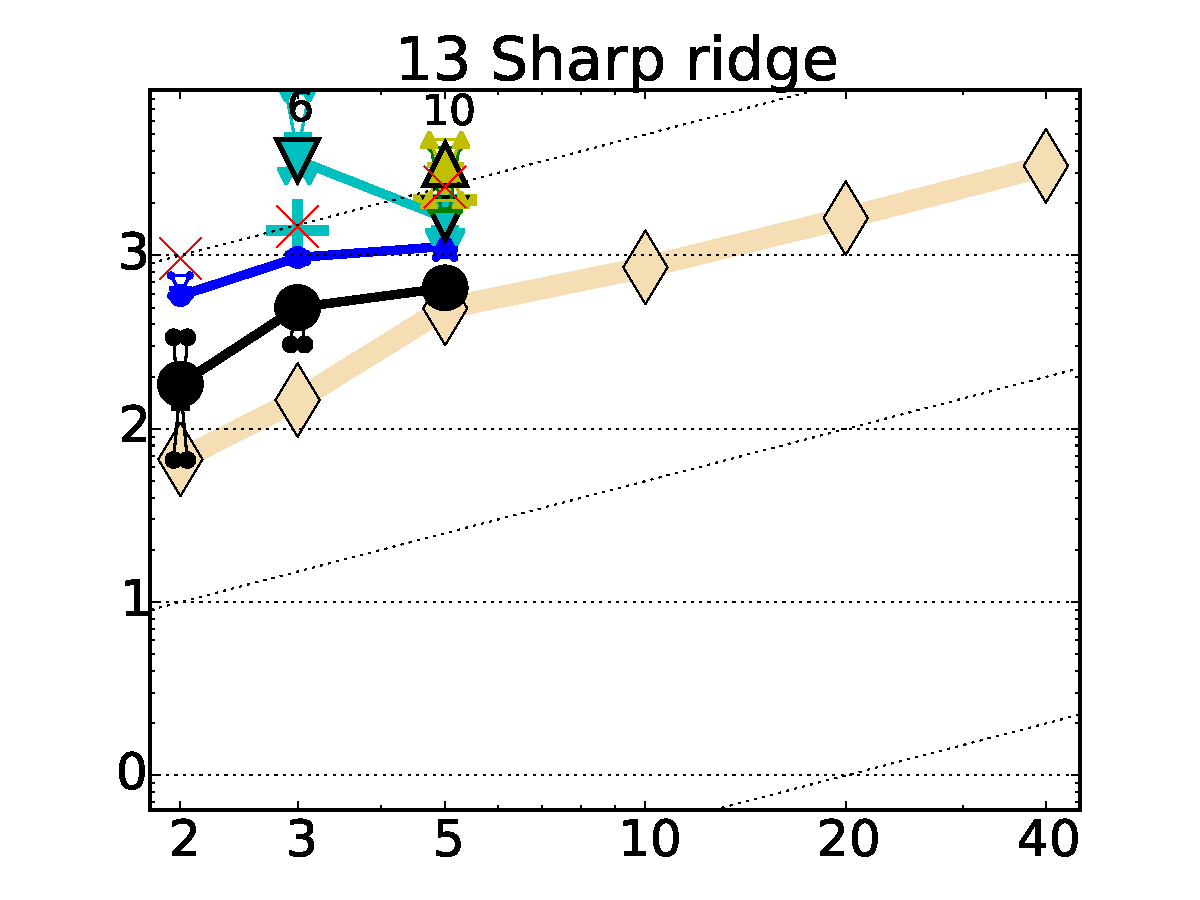
\includegraphics[width=0.268\textwidth]{ppfigdim_f013}&
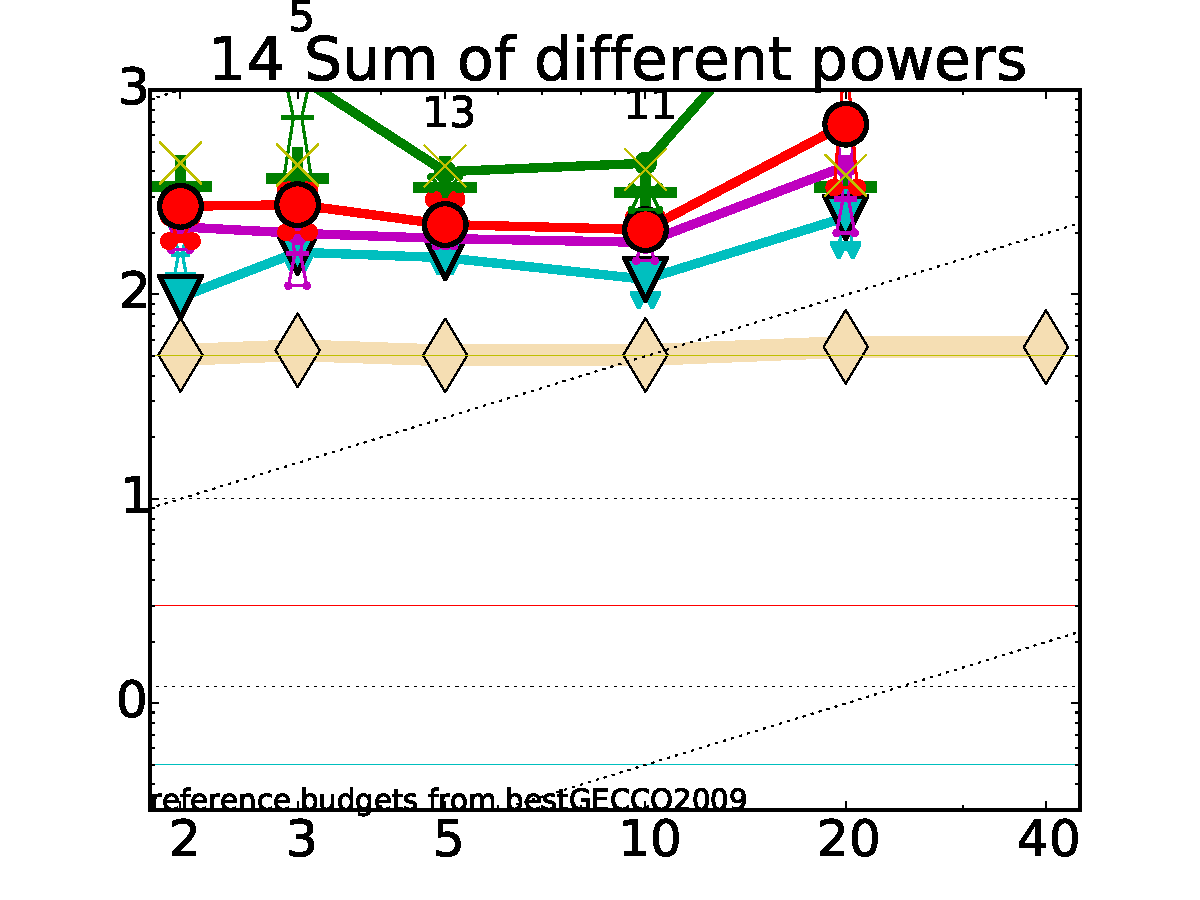
\includegraphics[width=0.268\textwidth]{ppfigdim_f014}&
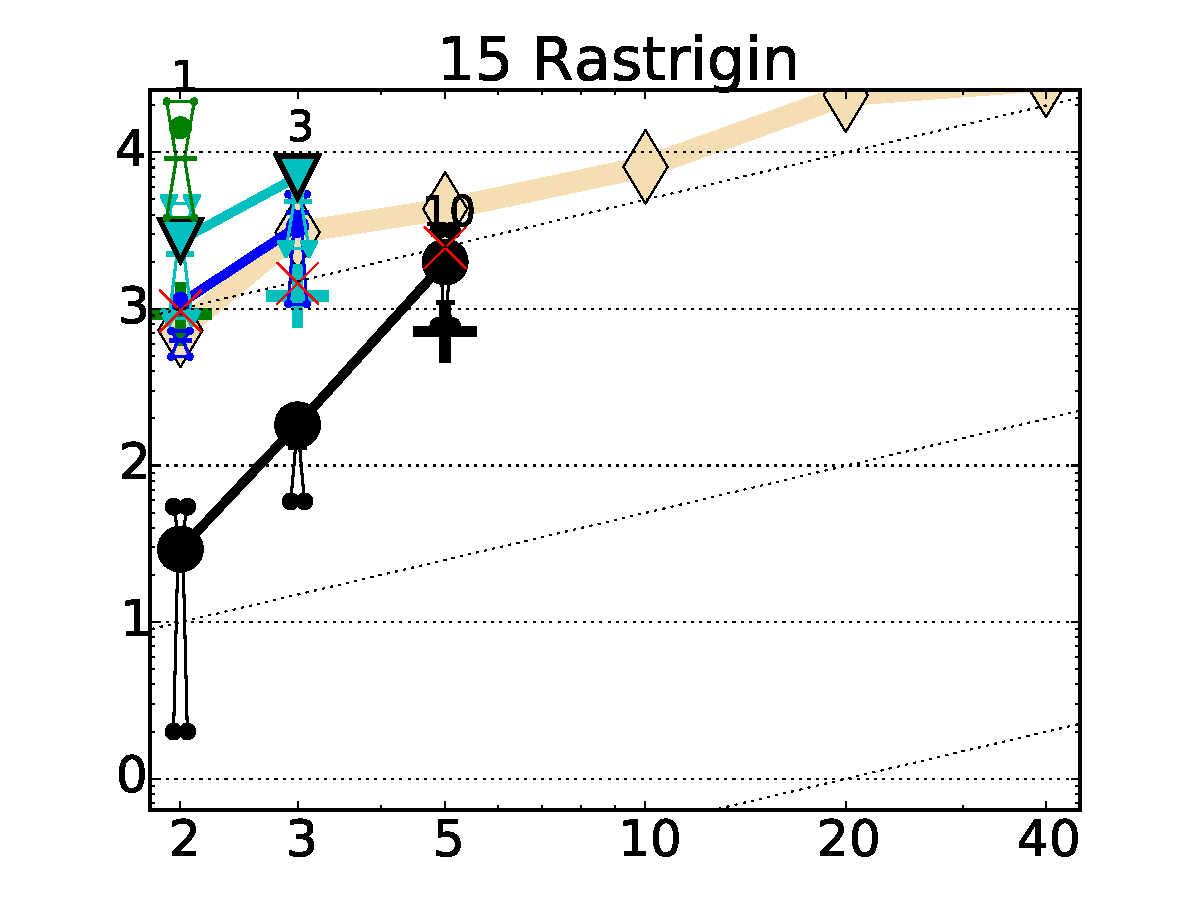
\includegraphics[width=0.268\textwidth]{ppfigdim_f015}&
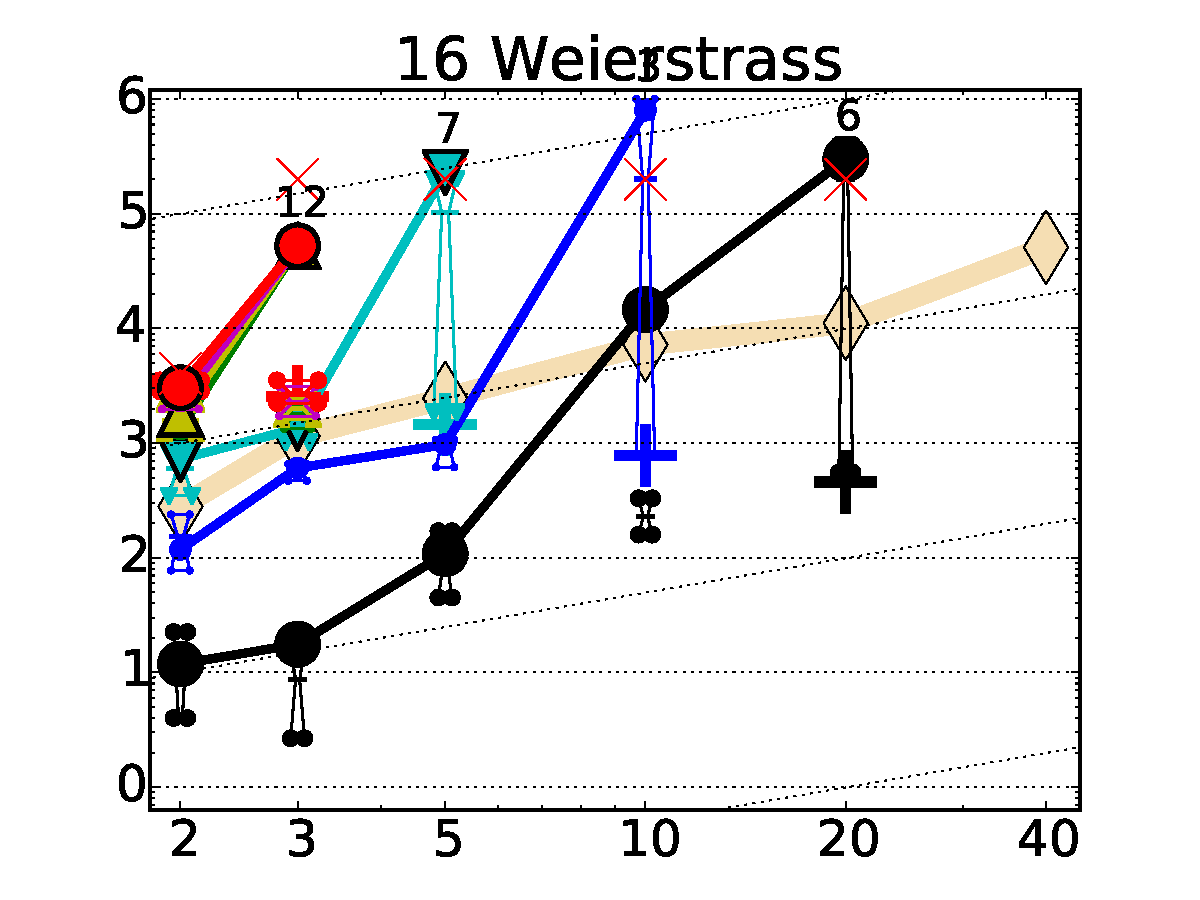
\includegraphics[width=0.268\textwidth]{ppfigdim_f016}\\[-2.2ex]
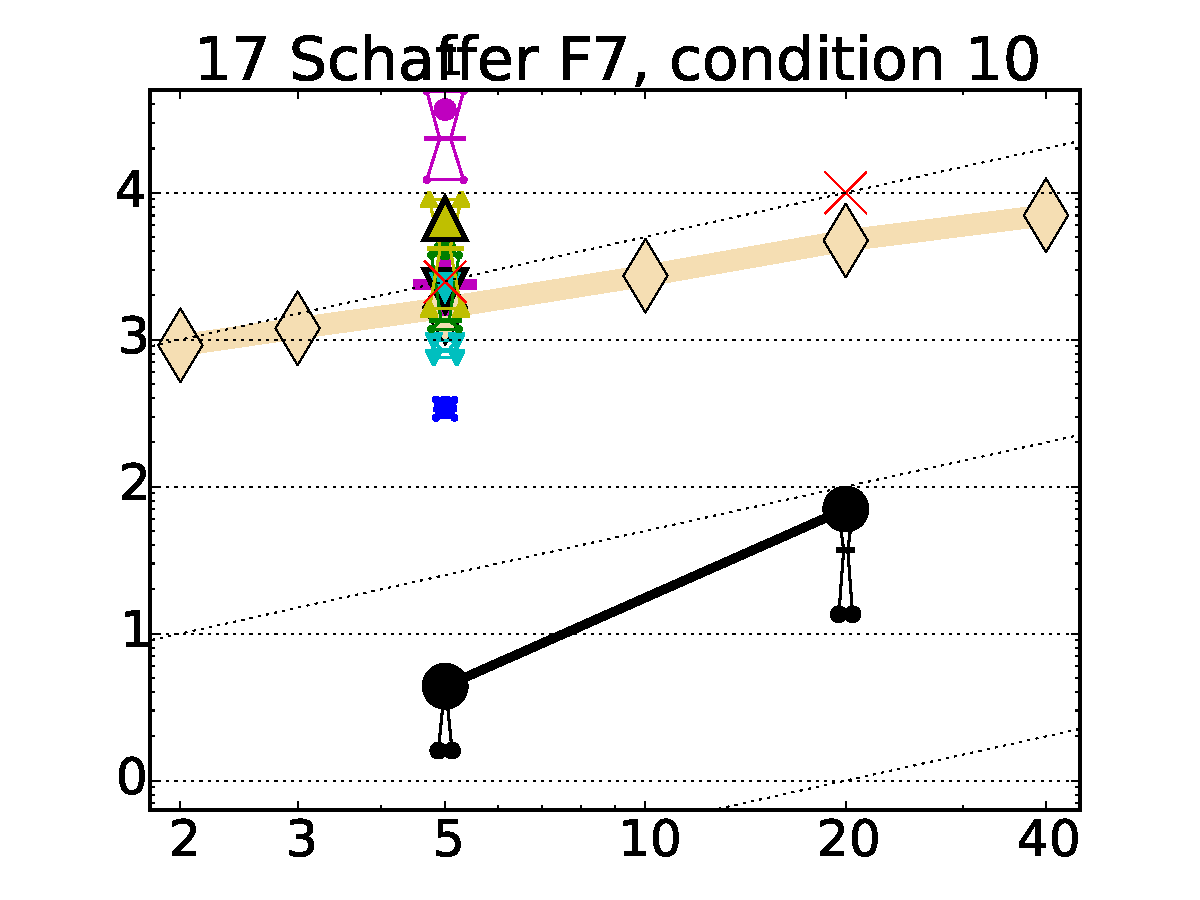
\includegraphics[width=0.268\textwidth]{ppfigdim_f017}&
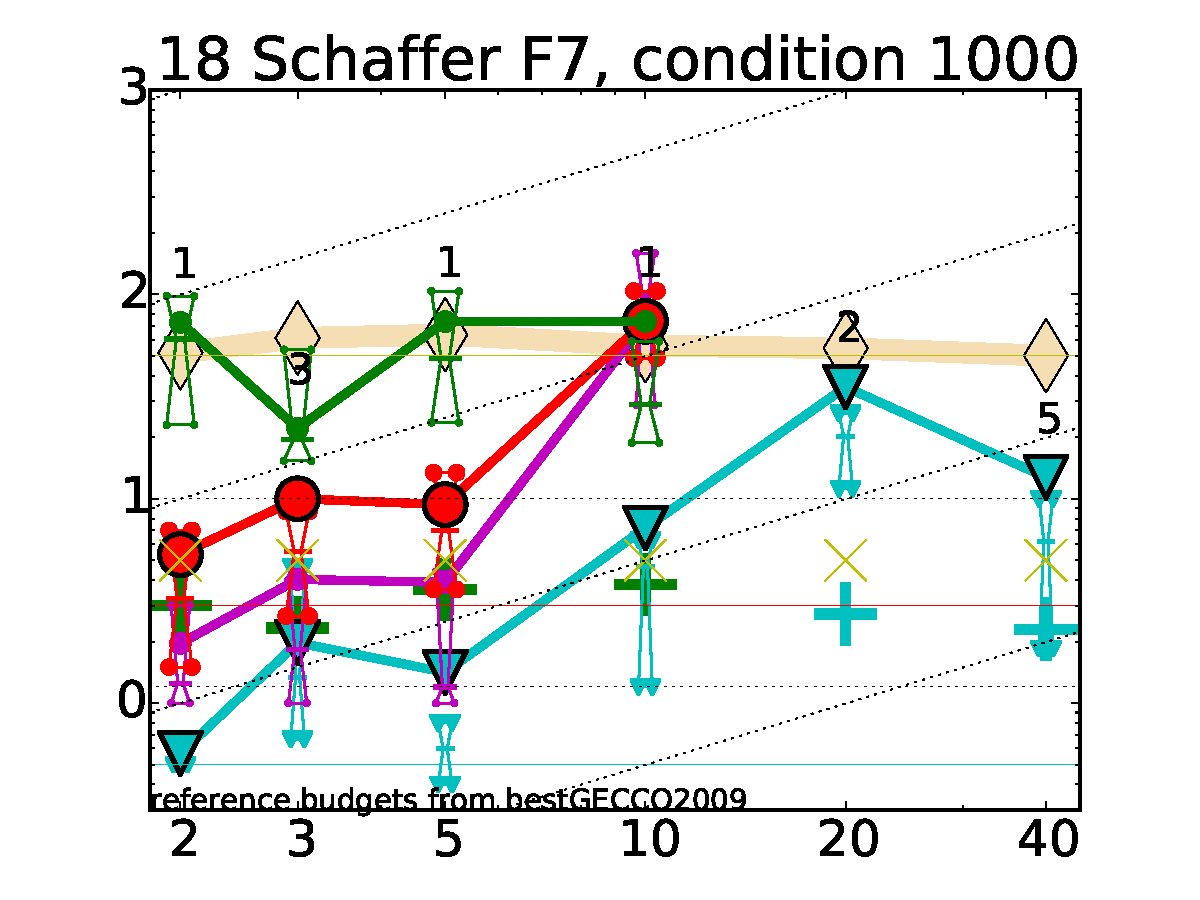
\includegraphics[width=0.268\textwidth]{ppfigdim_f018}&
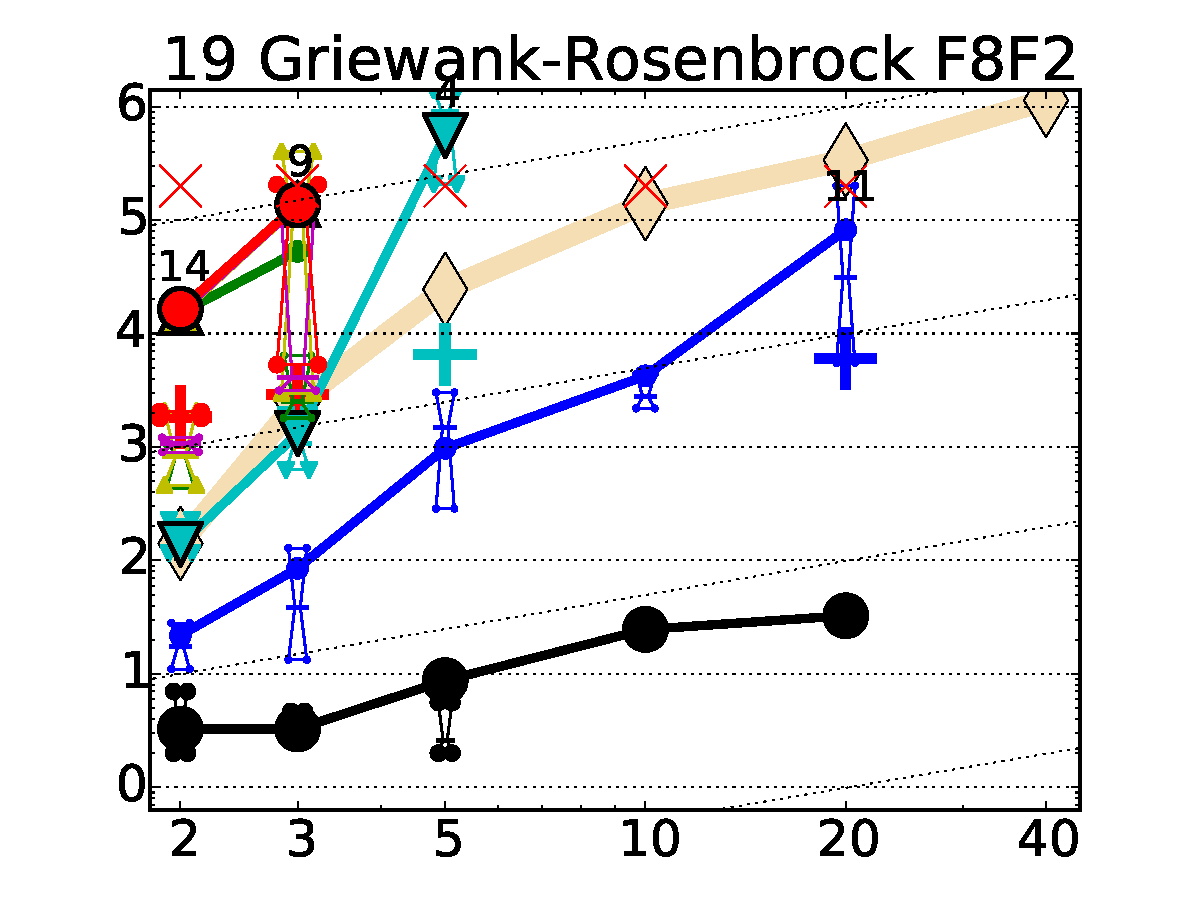
\includegraphics[width=0.268\textwidth]{ppfigdim_f019}&
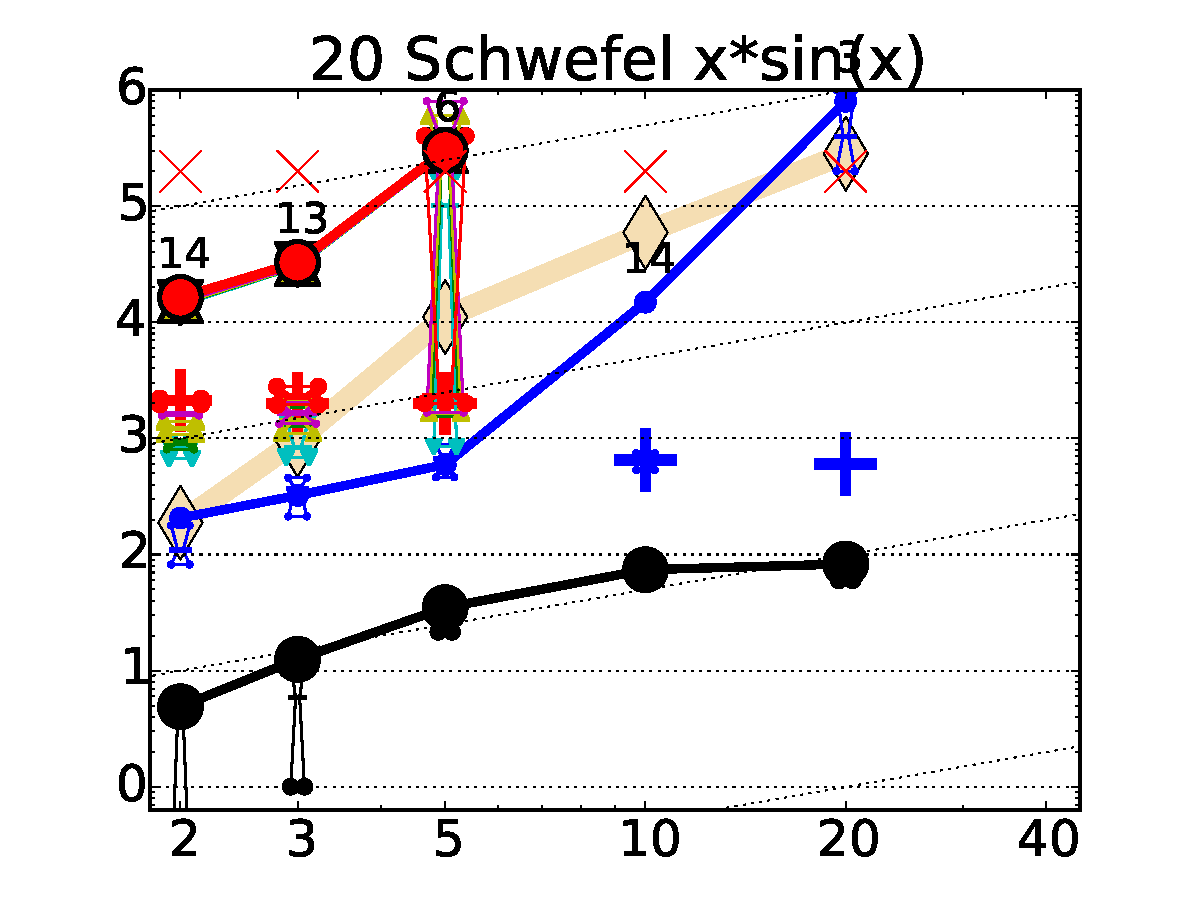
\includegraphics[width=0.268\textwidth]{ppfigdim_f020}\\[-2.2ex]
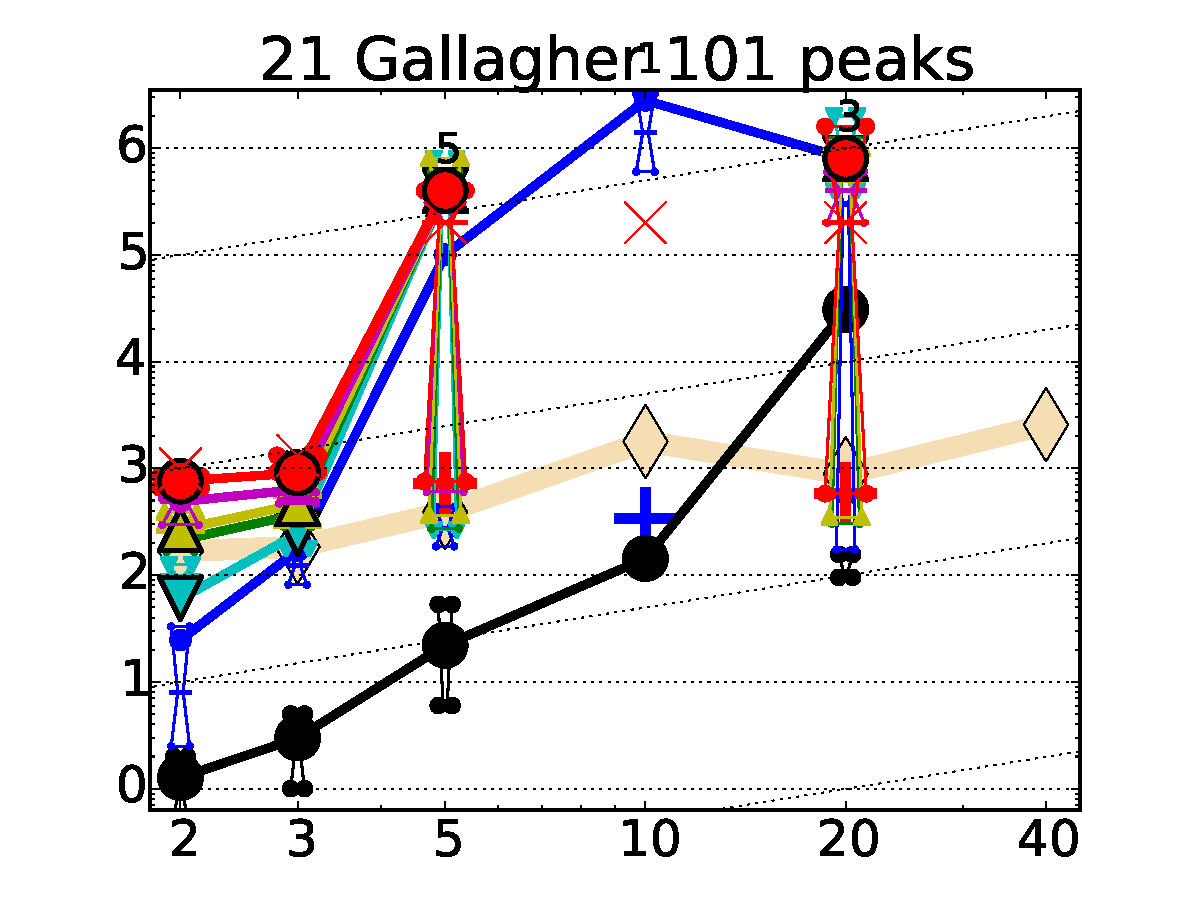
\includegraphics[width=0.268\textwidth]{ppfigdim_f021}&
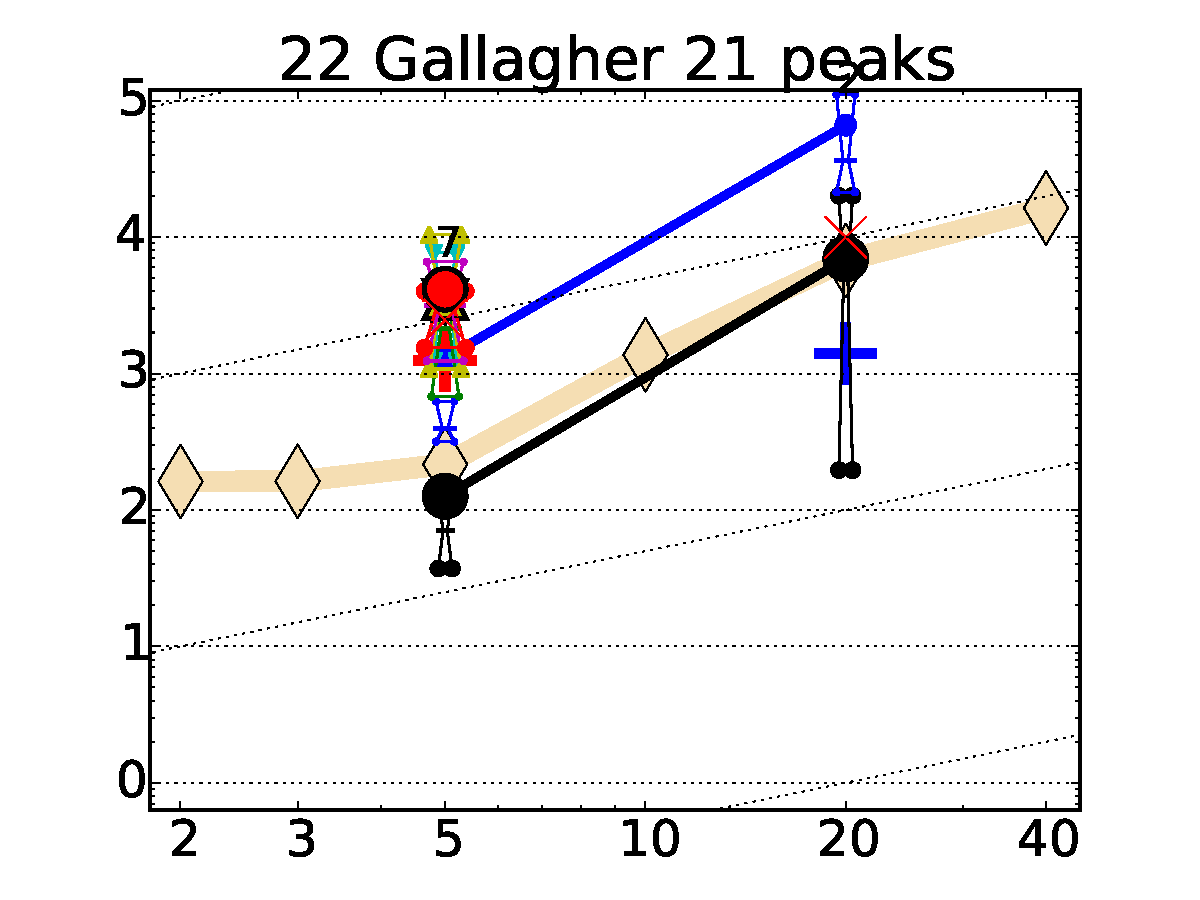
\includegraphics[width=0.268\textwidth]{ppfigdim_f022}&
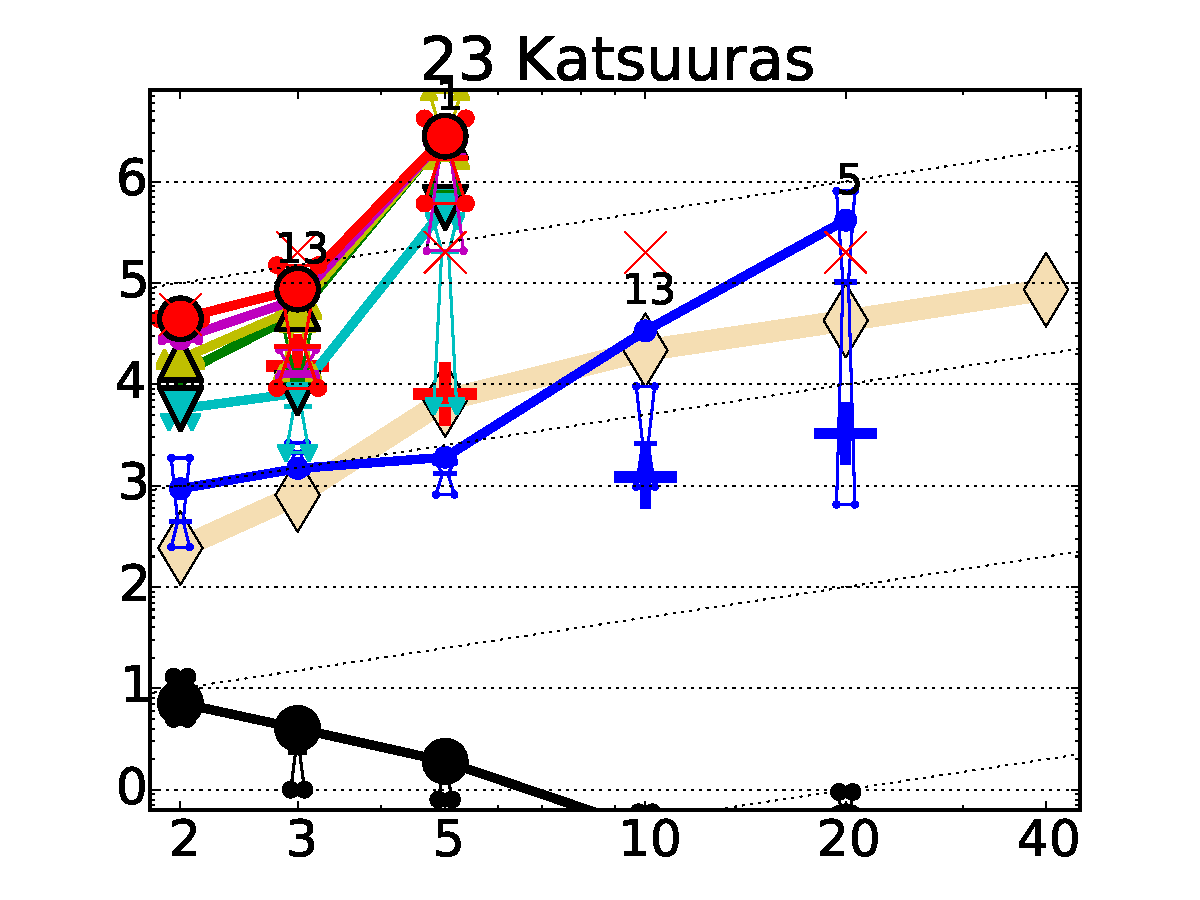
\includegraphics[width=0.268\textwidth]{ppfigdim_f023}&
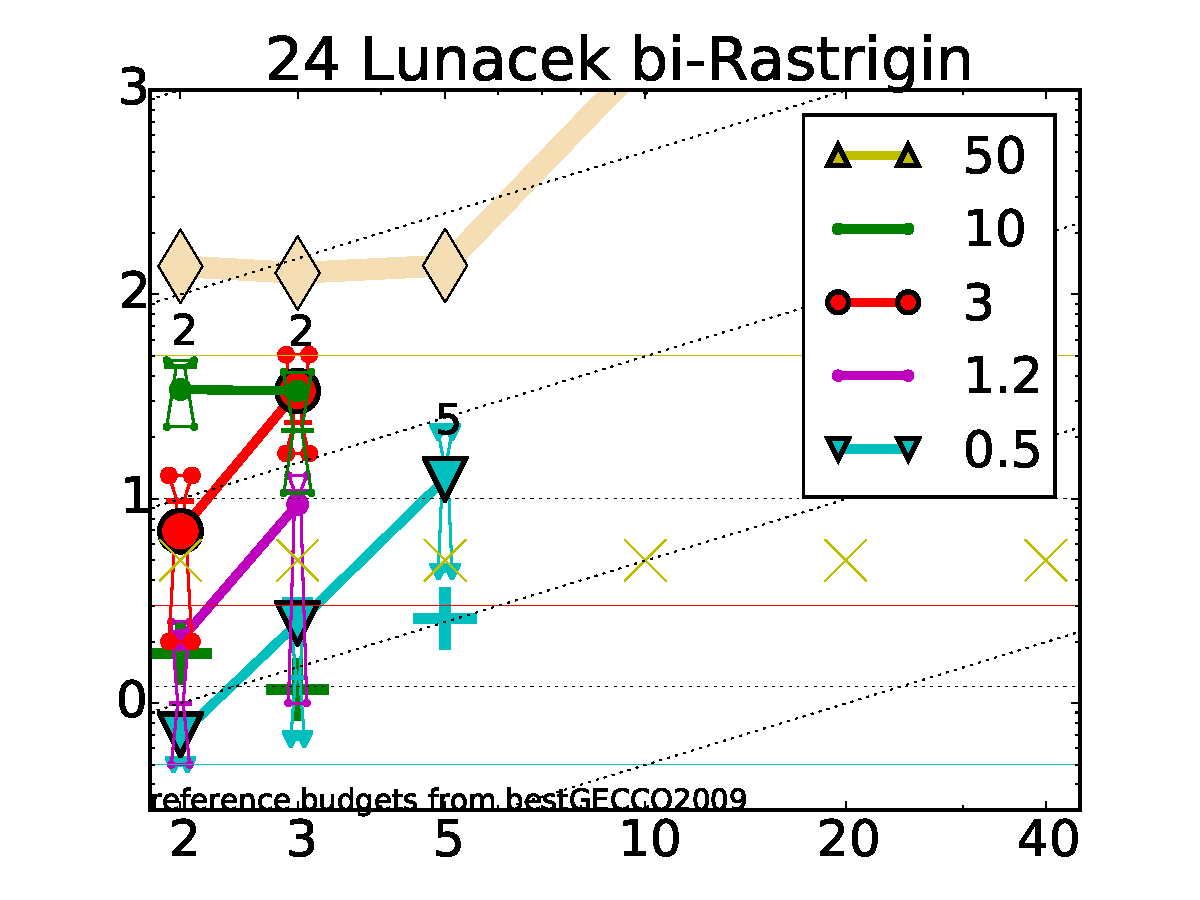
\includegraphics[width=0.268\textwidth]{ppfigdim_f024}
\end{tabular}
\vspace{-3ex}
 \caption{\label{fig:ERTgraphs}
 \bbobppfigdimlegend{$f_1$ and $f_{24}$}
 }
\end{figure*}

%%%%%%%%%%%%%%%%%%%%%%%%%%%%%%%%%%%%%%%%%%%%%%%%%%%%%%%%%%%%%%%%%%%%%%%%%%%%%%%
%%%%%%%%%%%%%%%%%%%%%%%%%%%%%%%%%%%%%%%%%%%%%%%%%%%%%%%%%%%%%%%%%%%%%%%%%%%%%%%
 
% Table showing the expected running time (ERT in number of function
% evaluations) divided by the best ERT measured during BBOB-2009 (given in the
% first row of each cell) for functions $f_1$--$f_{24}$.

%%%%%%%%%%%%%%%%%%%%%%%%%%%%%%%%%%%%%%%%%%%%%%%%%%%%%%%%%%%%%%%%%%%%%%%%%%%%%%%

\begin{table*}
\centering {\tiny
\parbox{0.499\textwidth}{\centering
   {\small 5-D}\\
   \input{\bbobdatapath\algfolder pptable_05D_noiselessall}}%
\parbox{0.499\textwidth}{\centering
   {\small 20-D}\\
   \input{\bbobdatapath\algfolder pptable_20D_noiselessall}}}%
\caption[Table of ERTs]{\label{tab:ERTs}\bbobpptablecaption{} 
}
\end{table*}
%%%%%%%%%%%%%%%%%%%%%%%%%%%%%%%%%%%%%%%%%%%%%%%%%%%%%%%%%%%%%%%%%%%%%%%%%%%%%%%
%%%%%%%%%%%%%%%%%%%%%%%%%%%%%%%%%%%%%%%%%%%%%%%%%%%%%%%%%%%%%%%%%%%%%%%%%%%%%%%


%%%%%%%%%%%%%%%%%%%%%%%%%%%%%%%%%%%%%%%%%%%%%%%%%%%%%%%%%%%%%%%%%%%%%%%%%%%%%%%
%%%%%%%%%%%%%%%%%%%%%%%%%%%%%%%%%%%%%%%%%%%%%%%%%%%%%%%%%%%%%%%%%%%%%%%%%%%%%%%

% Empirical cumulative distribution functions (ECDFs) per function group.

%%%%%%%%%%%%%%%%%%%%%%%%%%%%%%%%%%%%%%%%%%%%%%%%%%%%%%%%%%%%%%%%%%%%%%%%%%%%%%%
\newcommand{\rot}[2][2.5]{
  \hspace*{-3.5\baselineskip}%
  \begin{rotate}{90}\hspace{#1em}#2
  \end{rotate}}
\begin{figure*}
\begin{tabular}{l@{\hspace*{-0.025\textwidth}}l@{\hspace*{-0.00\textwidth}}|l@{\hspace*{-0.025\textwidth}}l}
\multicolumn{2}{c}{$D=5$} & \multicolumn{2}{c}{$D=20$}\\[-0.5ex]
\rot{separable fcts}
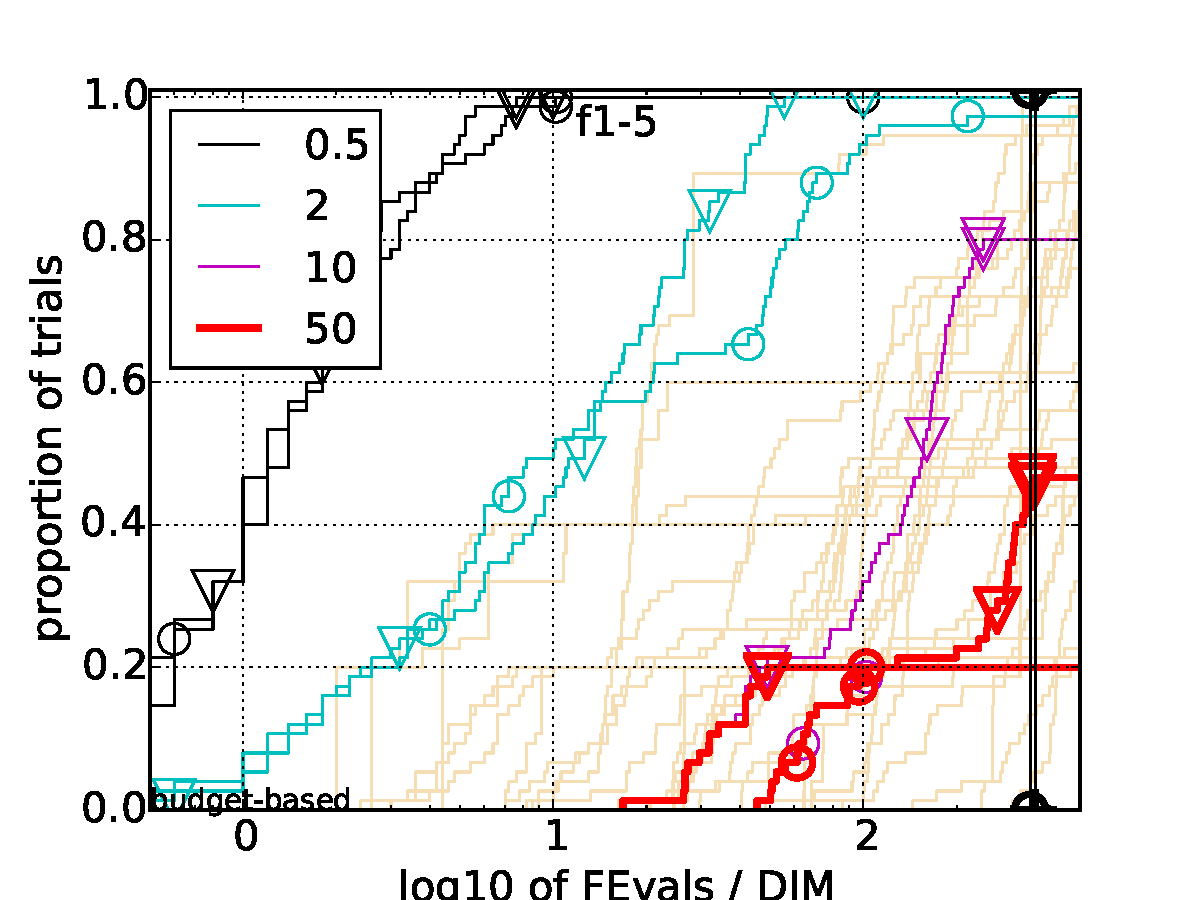
\includegraphics[width=0.268\textwidth,trim=0 0 0 13mm, clip]{pprldistr_05D_separ} &
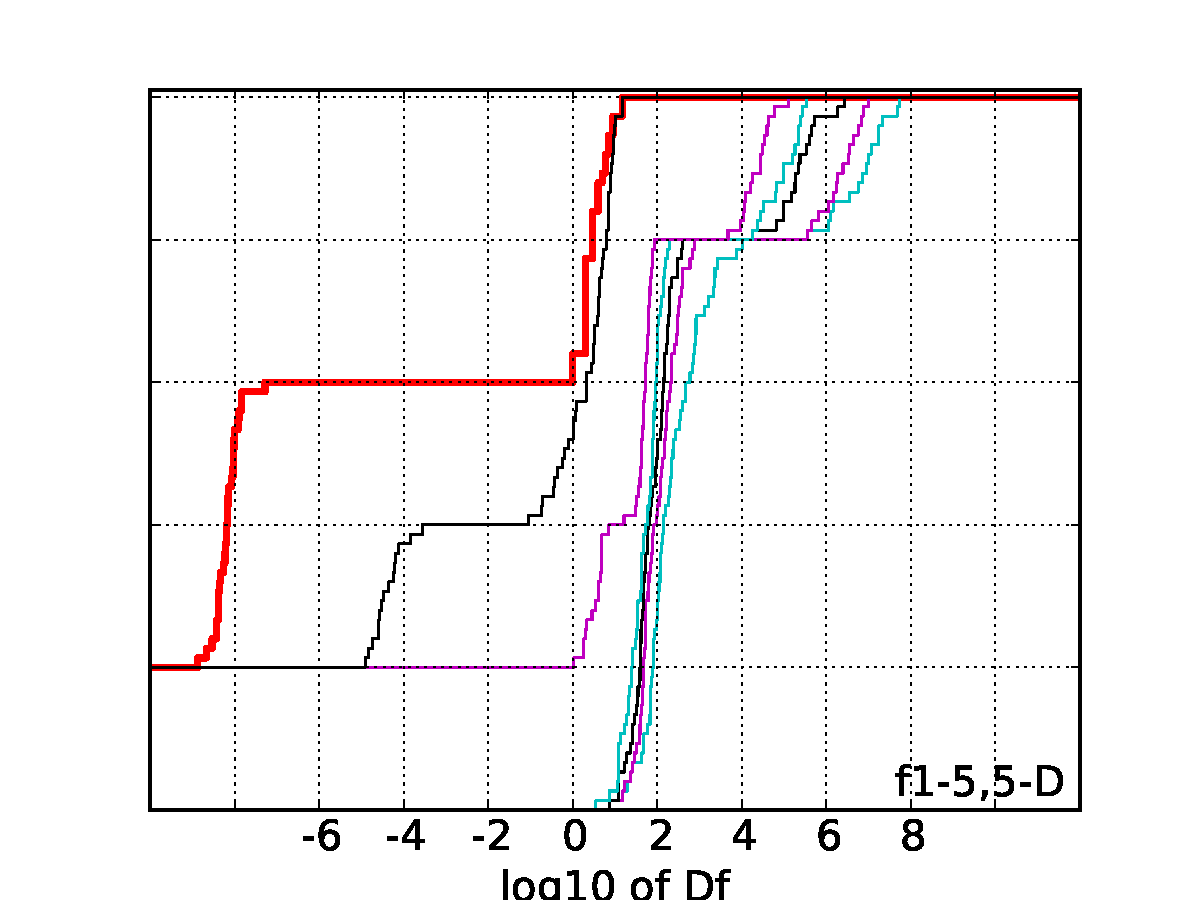
\includegraphics[width=0.2362\textwidth,trim=2.40cm 0 0 13mm, clip]{ppfvdistr_05D_separ} &
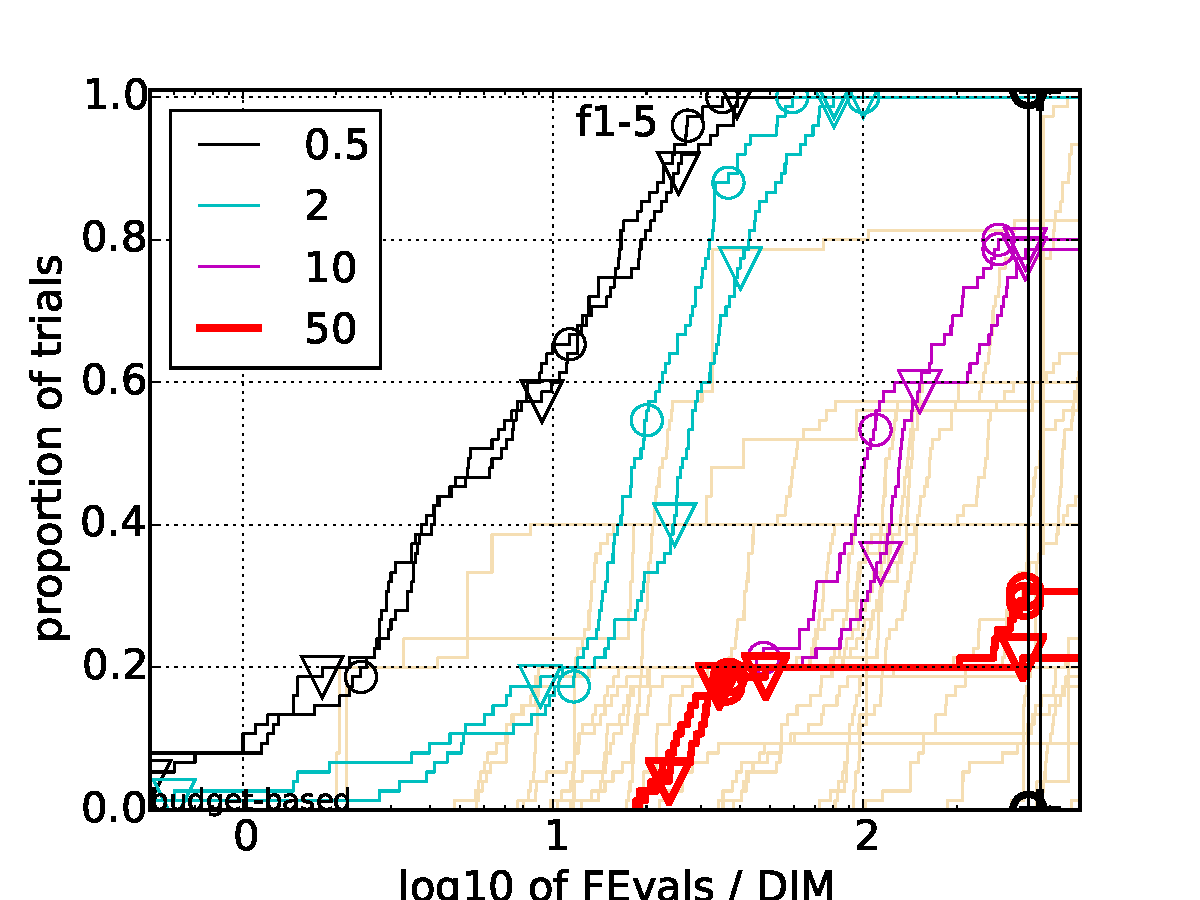
\includegraphics[width=0.268\textwidth,trim=0 0 0 13mm, clip]{pprldistr_20D_separ} &
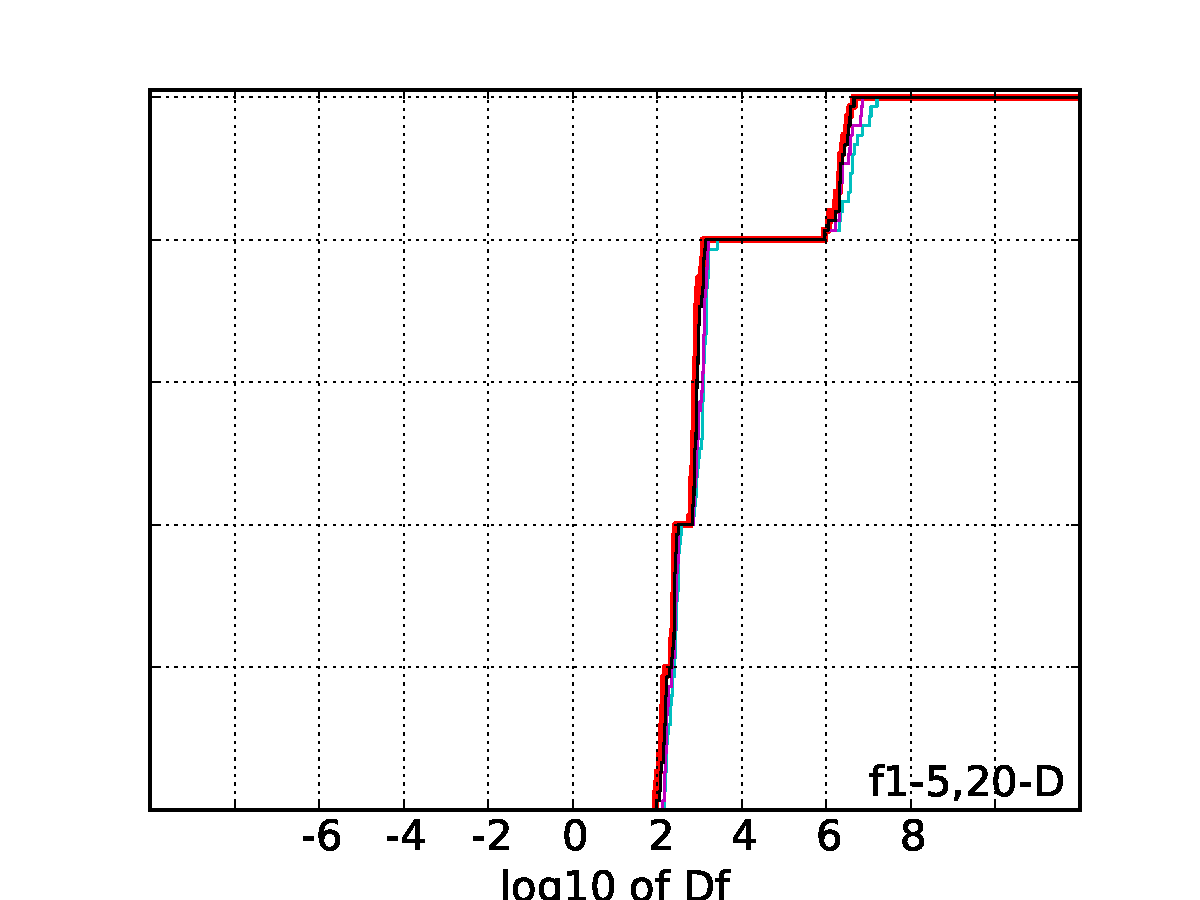
\includegraphics[width=0.2362\textwidth,trim=2.40cm 0 0 13mm, clip]{ppfvdistr_20D_separ} \\[-2ex]
\rot[1]{misc.\ moderate fcts}
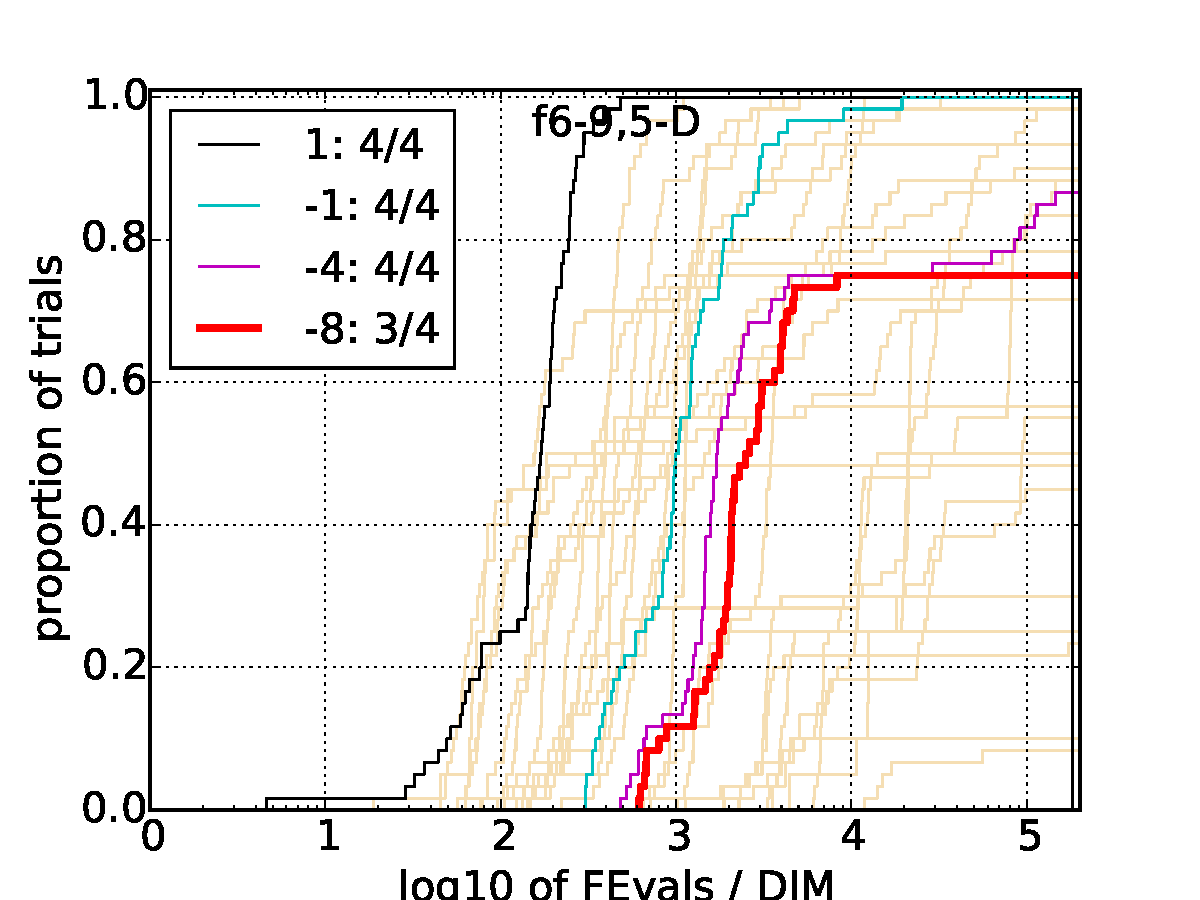
\includegraphics[width=0.268\textwidth,trim=0 0 0 13mm, clip]{pprldistr_05D_lcond} &
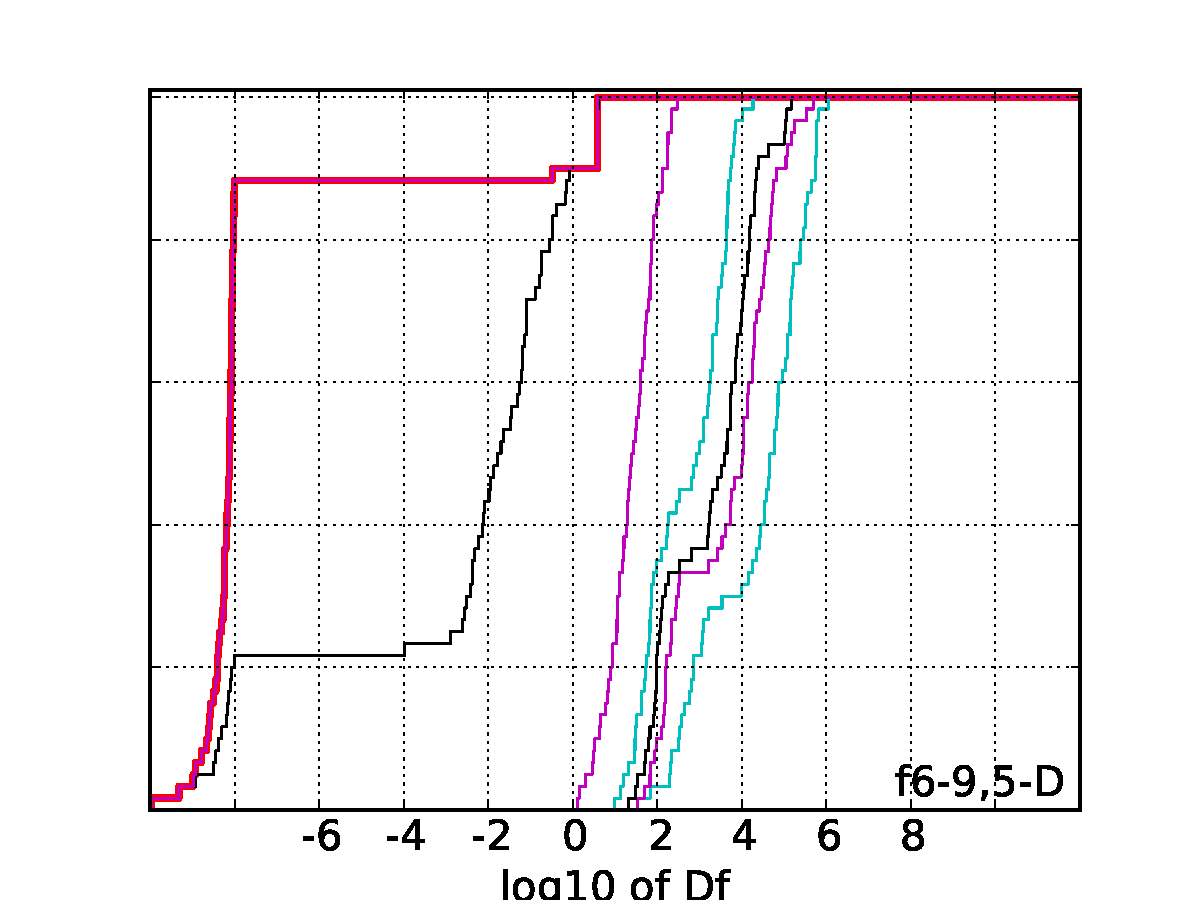
\includegraphics[width=0.2362\textwidth,trim=2.40cm 0 0 13mm, clip]{ppfvdistr_05D_lcond} &
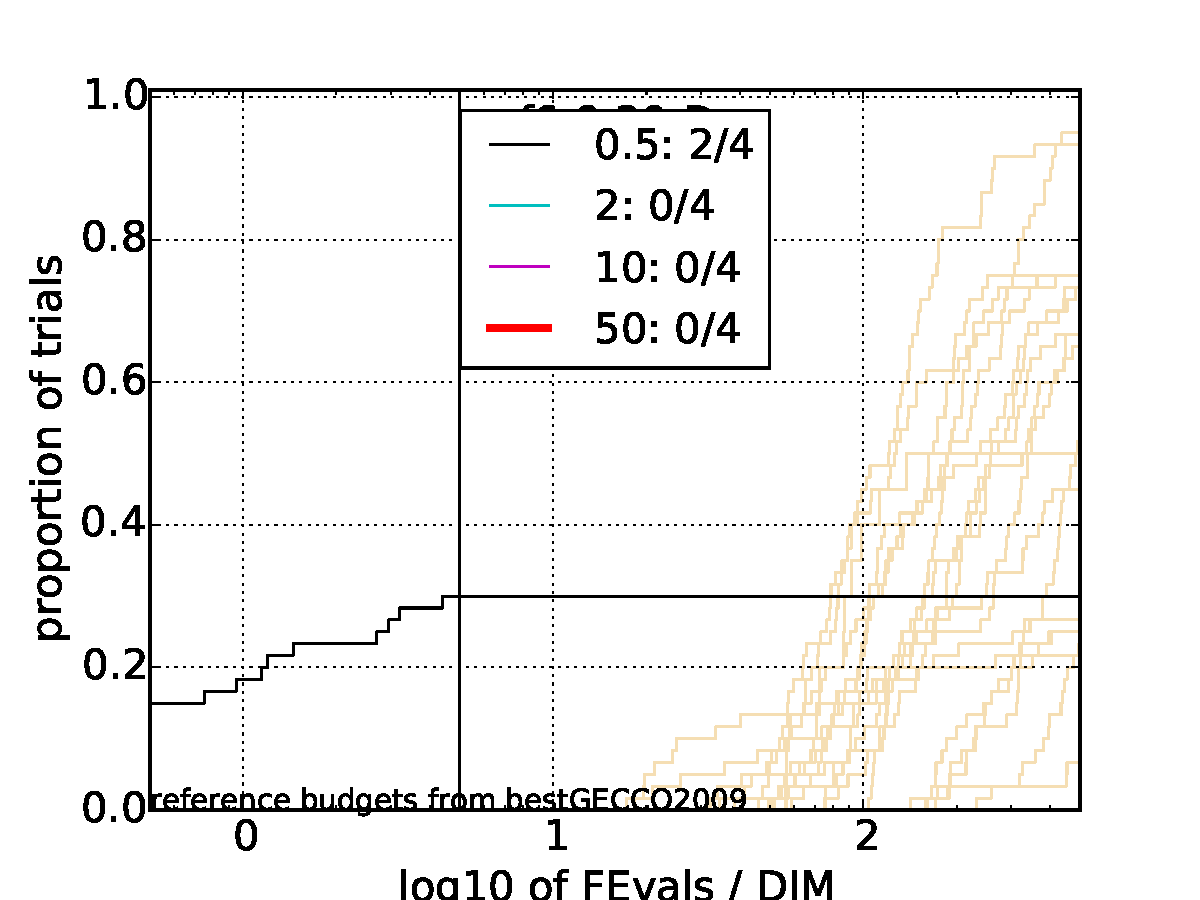
\includegraphics[width=0.268\textwidth,trim=0 0 0 13mm, clip]{pprldistr_20D_lcond} &
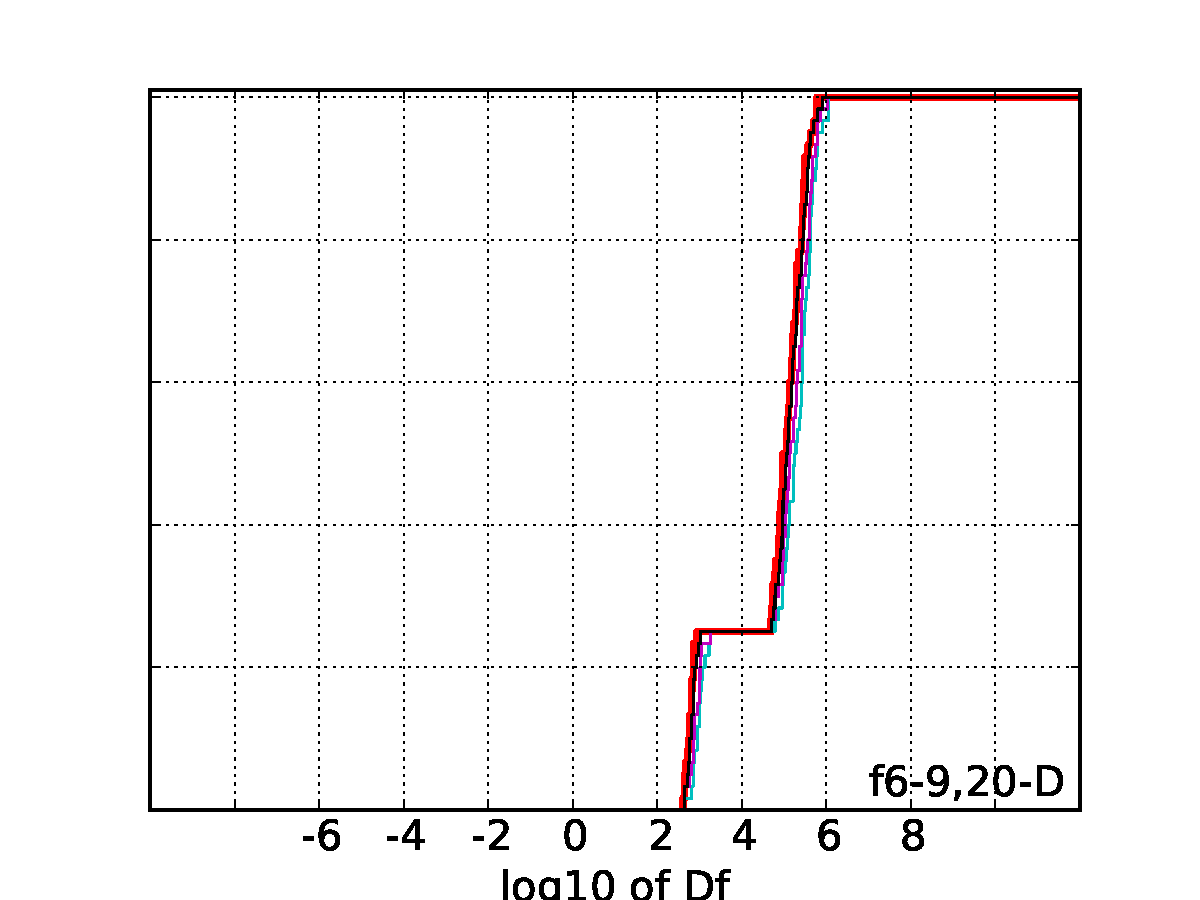
\includegraphics[width=0.2362\textwidth,trim=2.40cm 0 0 13mm, clip]{ppfvdistr_20D_lcond} \\[-2ex]
\rot[1.3]{ill-conditioned fcts}
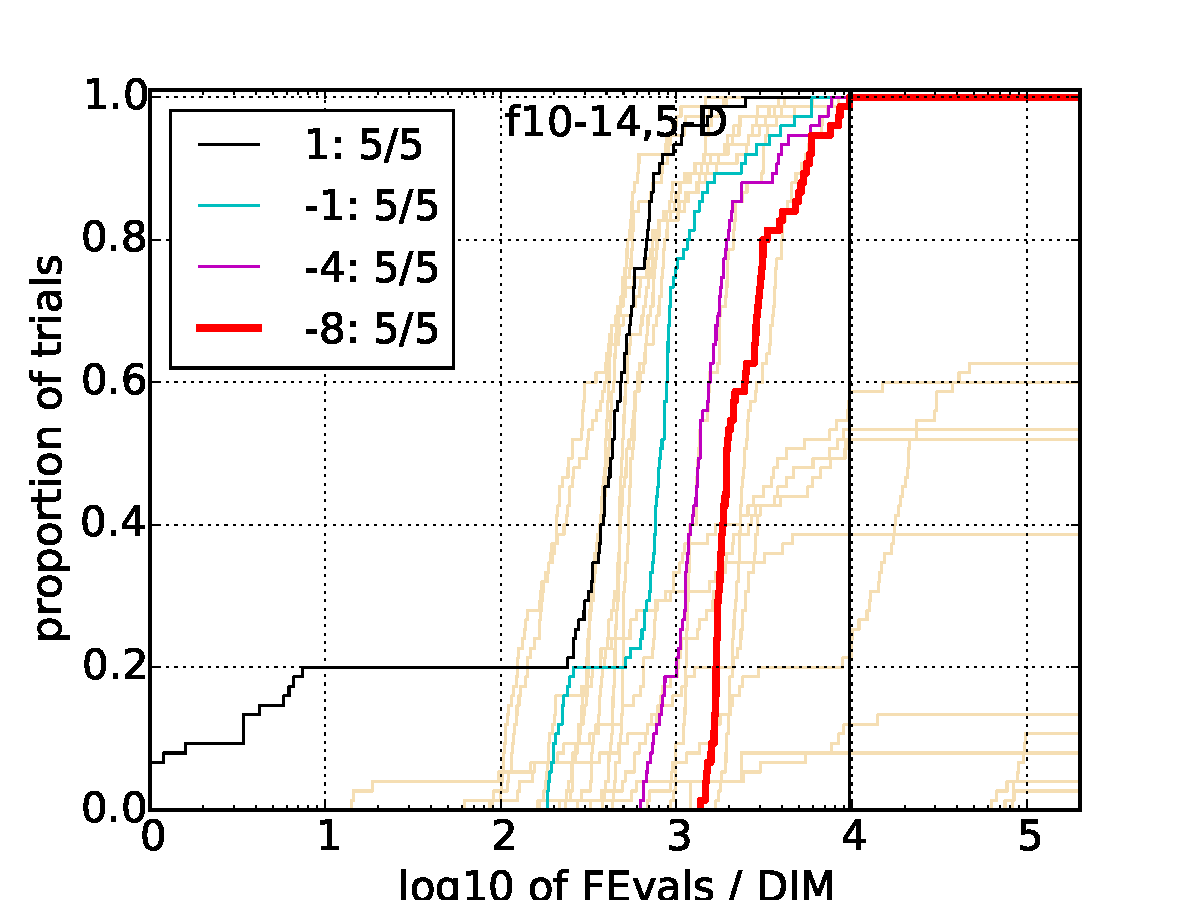
\includegraphics[width=0.268\textwidth,trim=0 0 0 13mm, clip]{pprldistr_05D_hcond} &
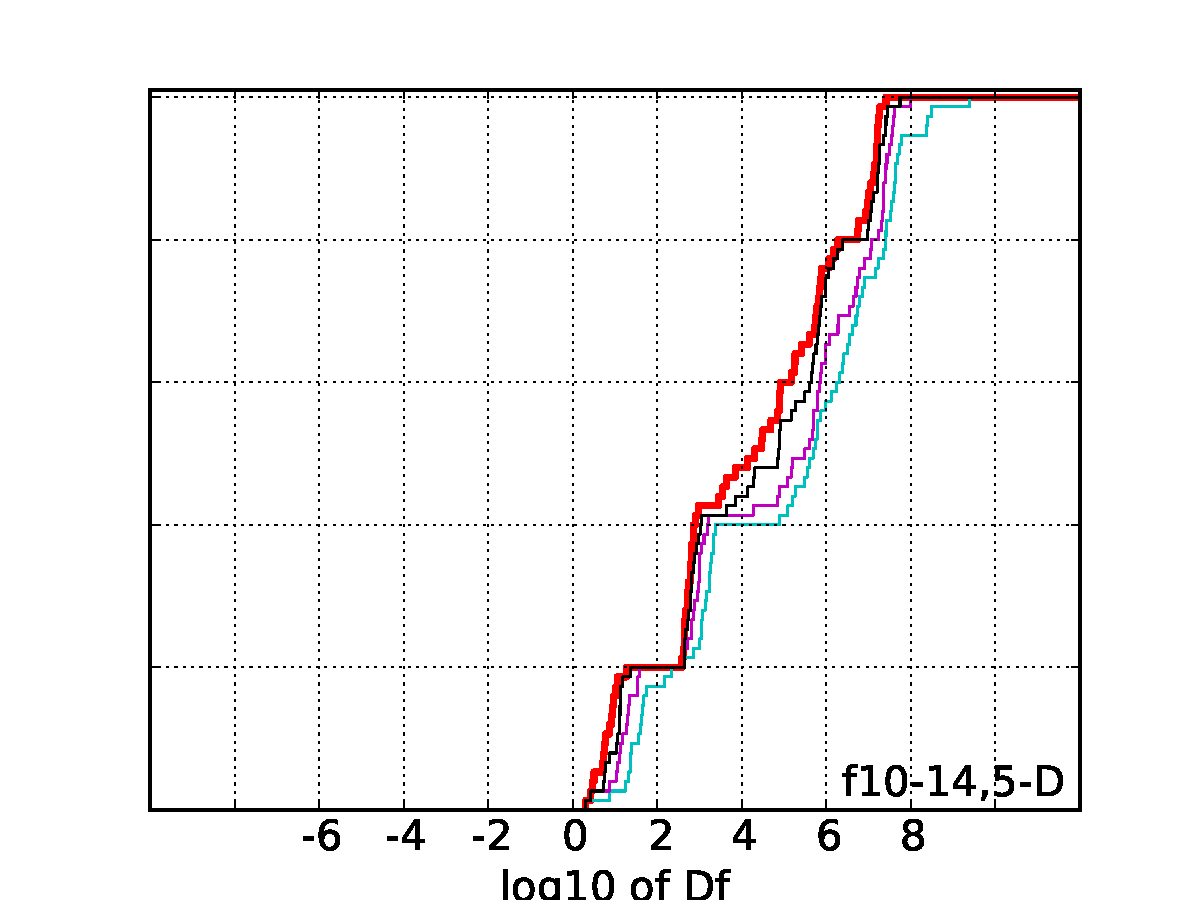
\includegraphics[width=0.2362\textwidth,trim=2.40cm 0 0 13mm, clip]{ppfvdistr_05D_hcond} &
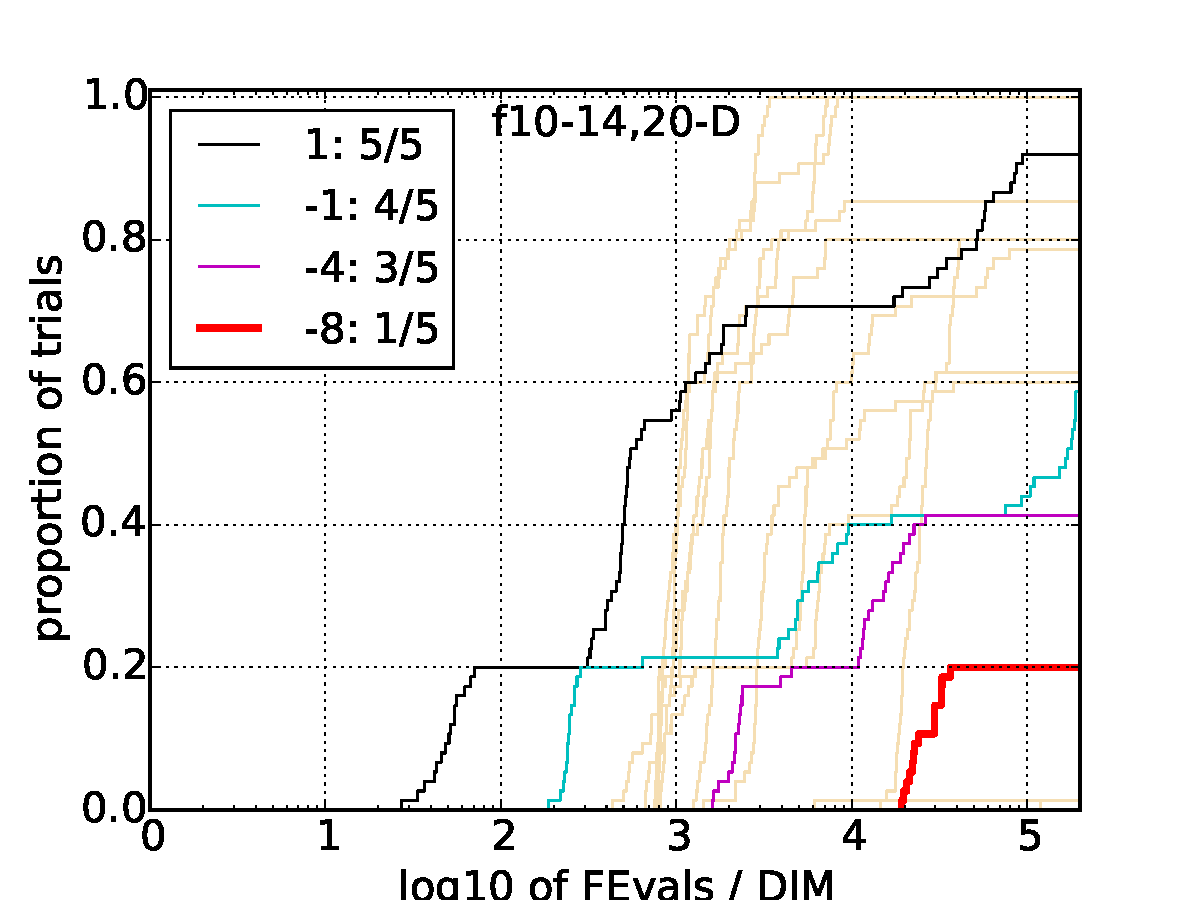
\includegraphics[width=0.268\textwidth,trim=0 0 0 13mm, clip]{pprldistr_20D_hcond} &
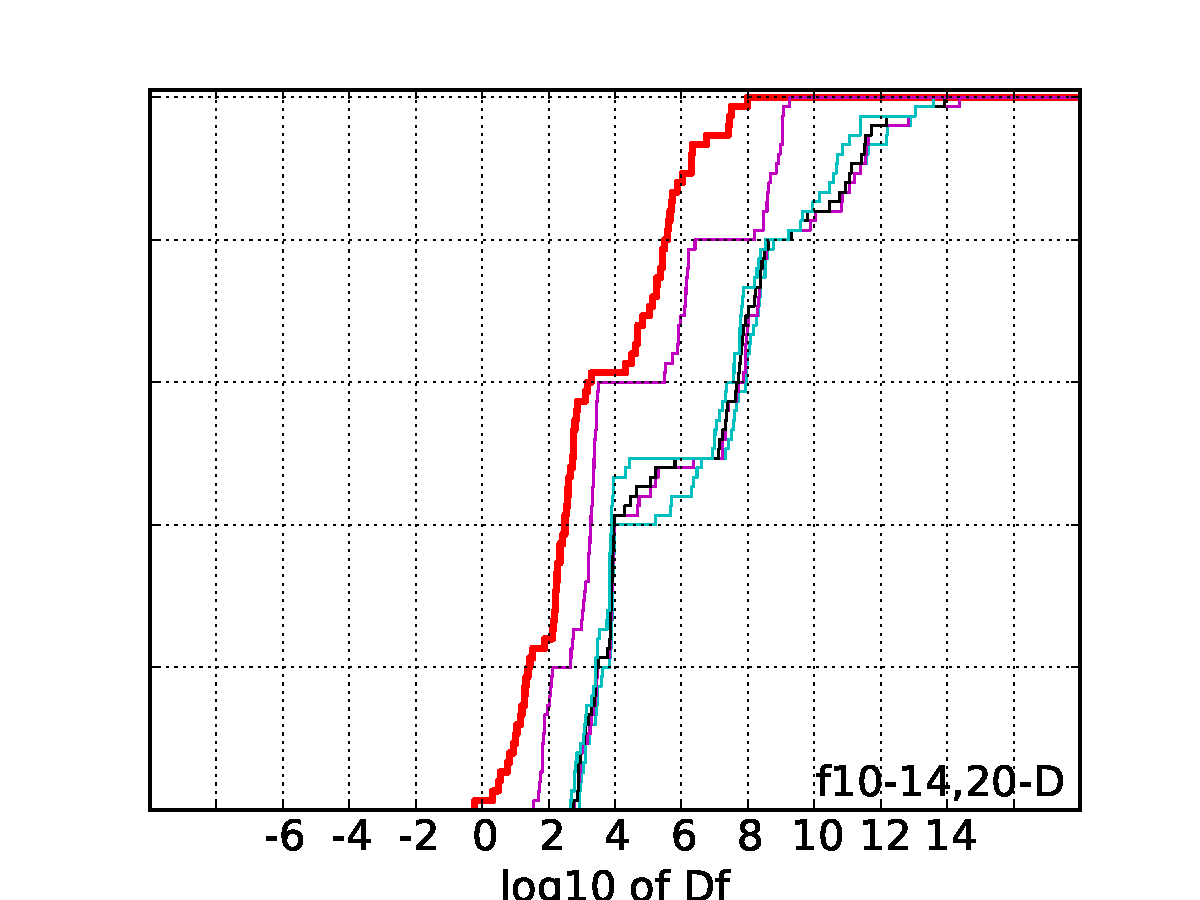
\includegraphics[width=0.2362\textwidth,trim=2.40cm 0 0 13mm, clip]{ppfvdistr_20D_hcond} \\[-2ex]
\rot[1.6]{multi-modal fcts}
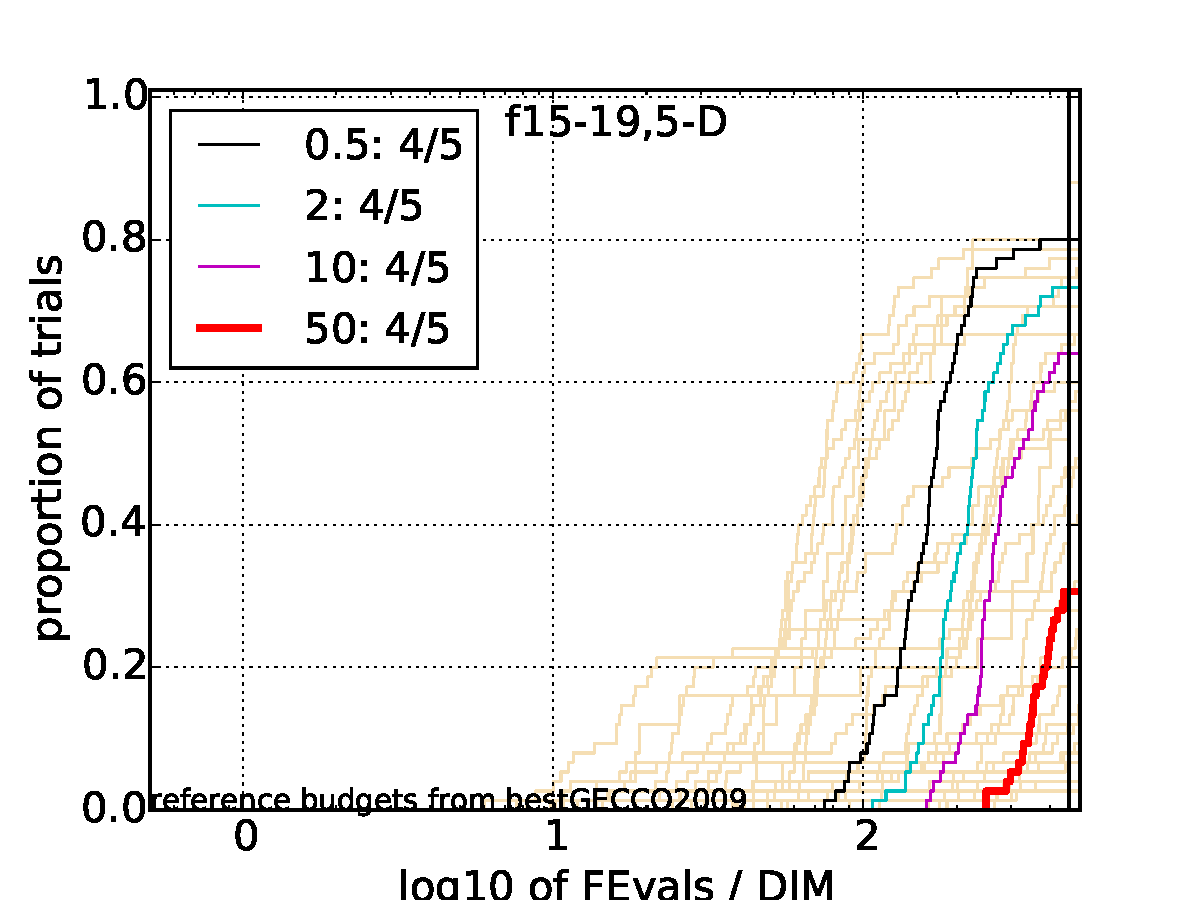
\includegraphics[width=0.268\textwidth,trim=0 0 0 13mm, clip]{pprldistr_05D_multi} &
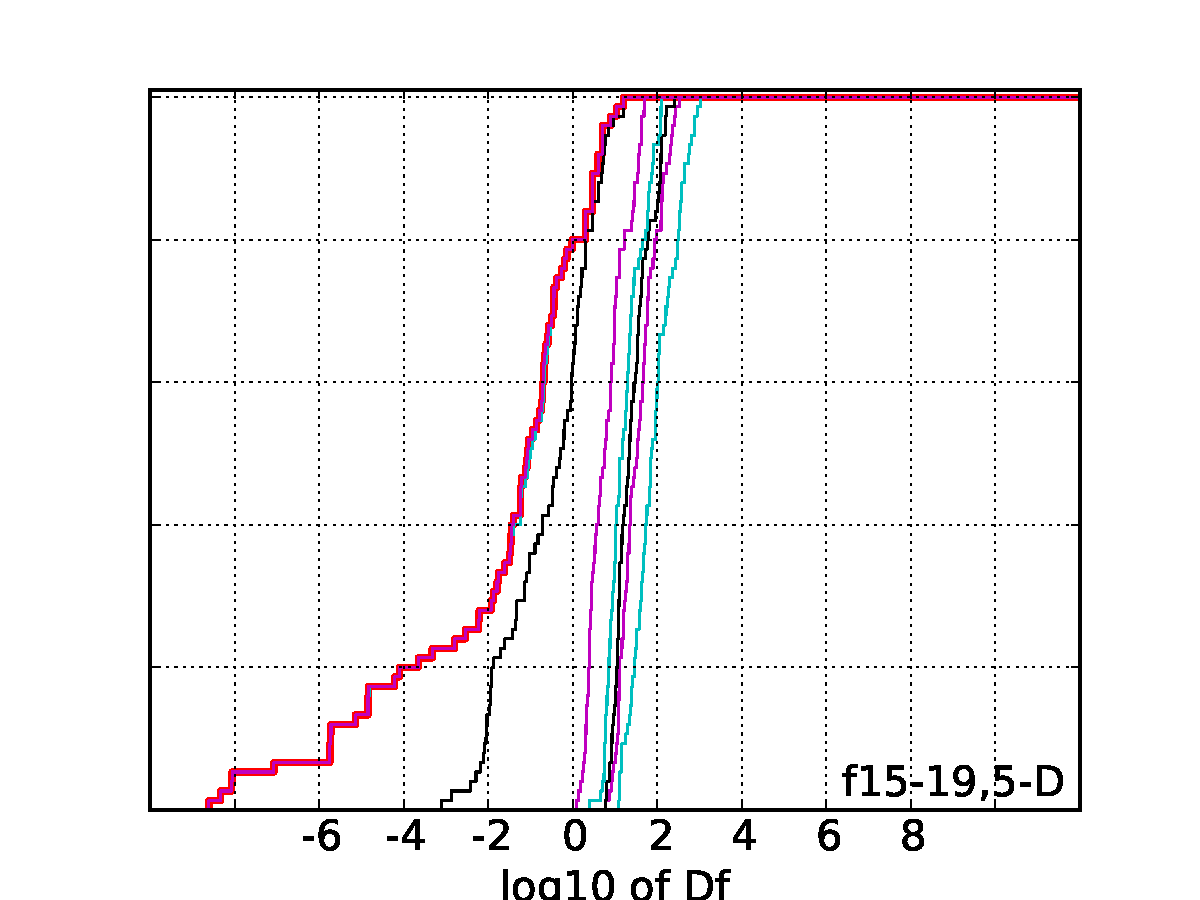
\includegraphics[width=0.2362\textwidth,trim=2.40cm 0 0 13mm, clip]{ppfvdistr_05D_multi} &
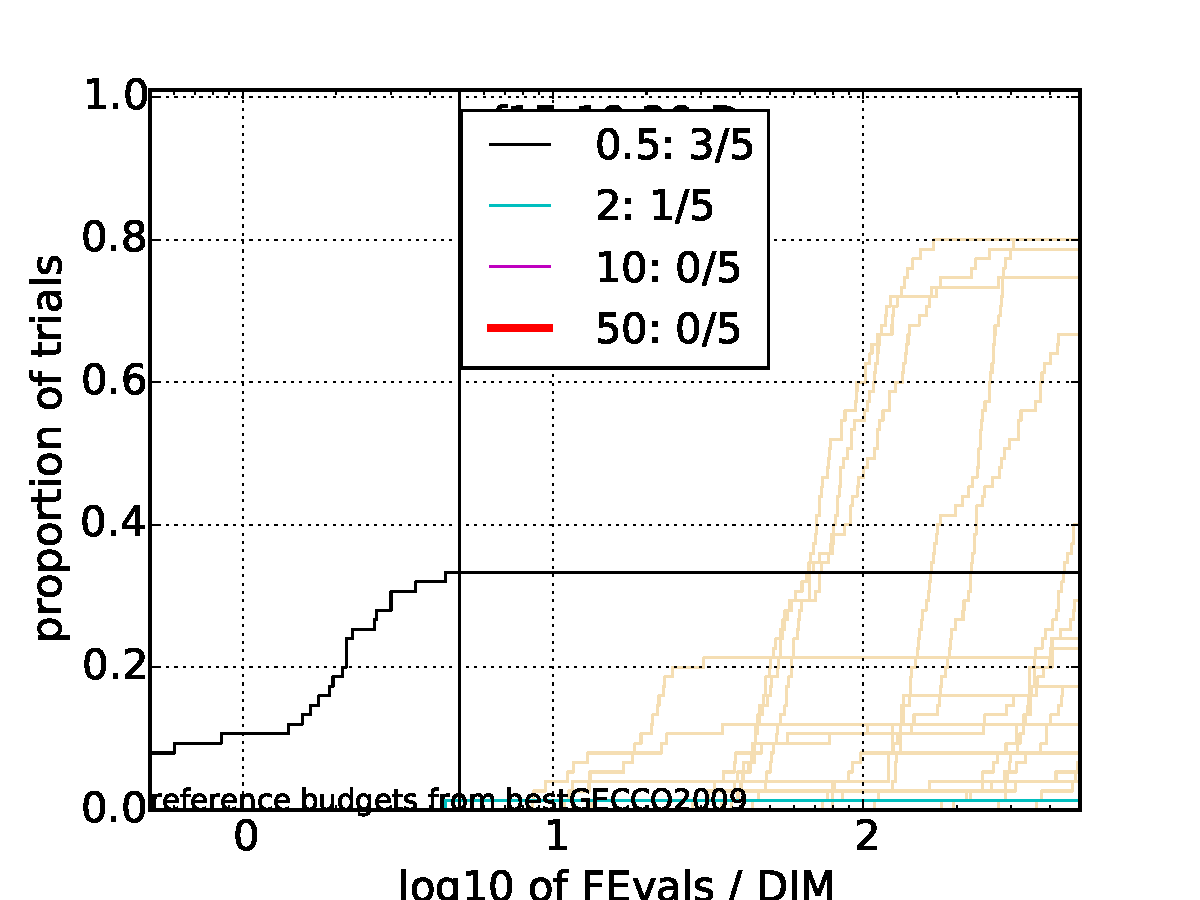
\includegraphics[width=0.268\textwidth,trim=0 0 0 13mm, clip]{pprldistr_20D_multi} &
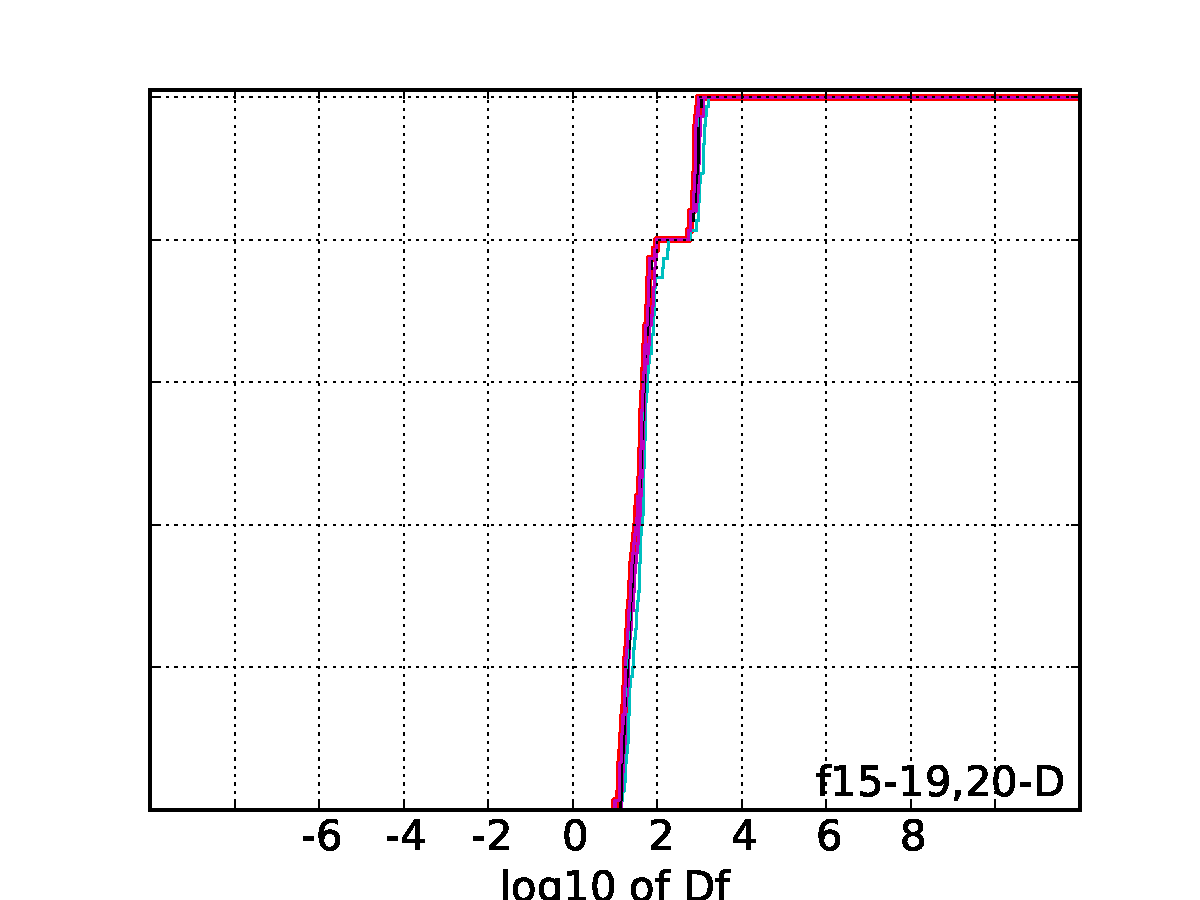
\includegraphics[width=0.2362\textwidth,trim=2.40cm 0 0 13mm, clip]{ppfvdistr_20D_multi} \\[-2ex]
\rot[1.0]{weak structure fcts}
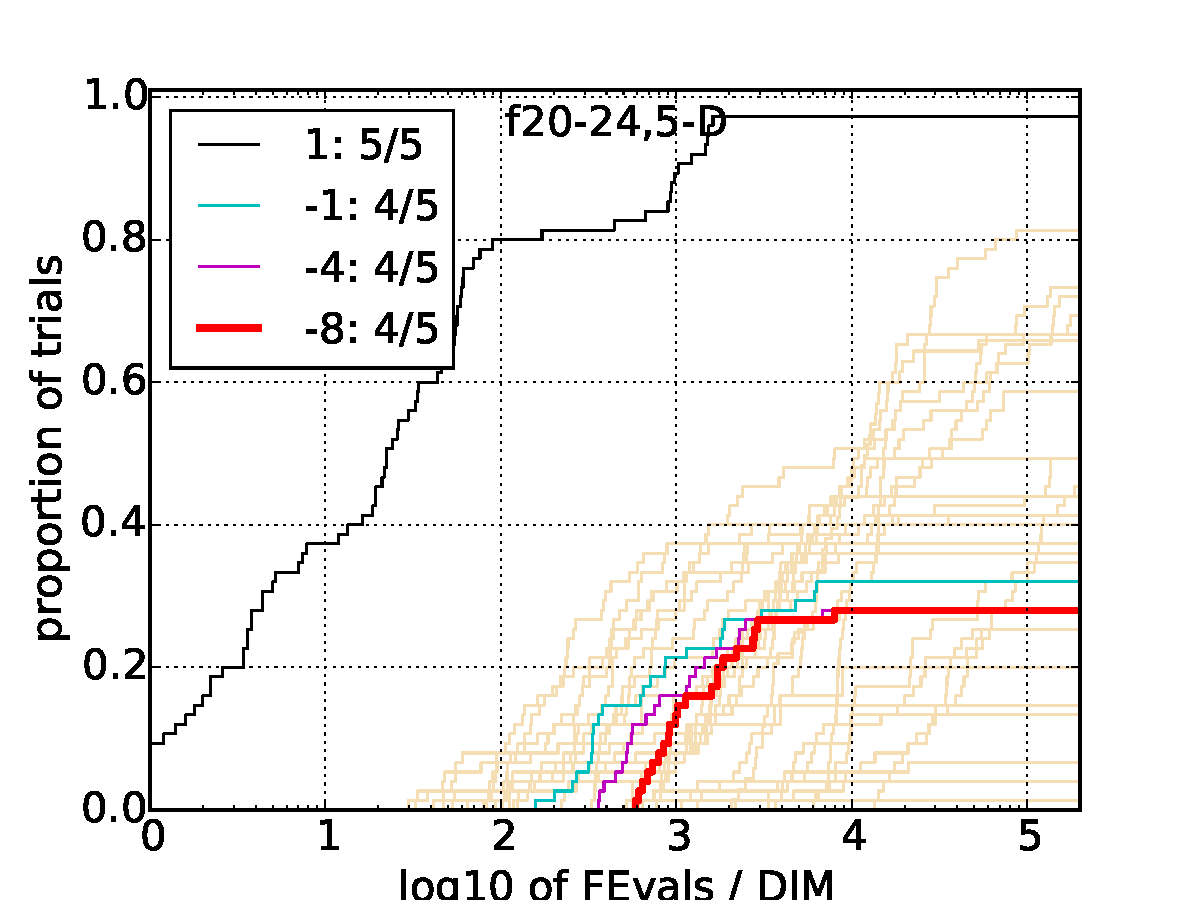
\includegraphics[width=0.268\textwidth,trim=0 0 0 13mm, clip]{pprldistr_05D_mult2} &
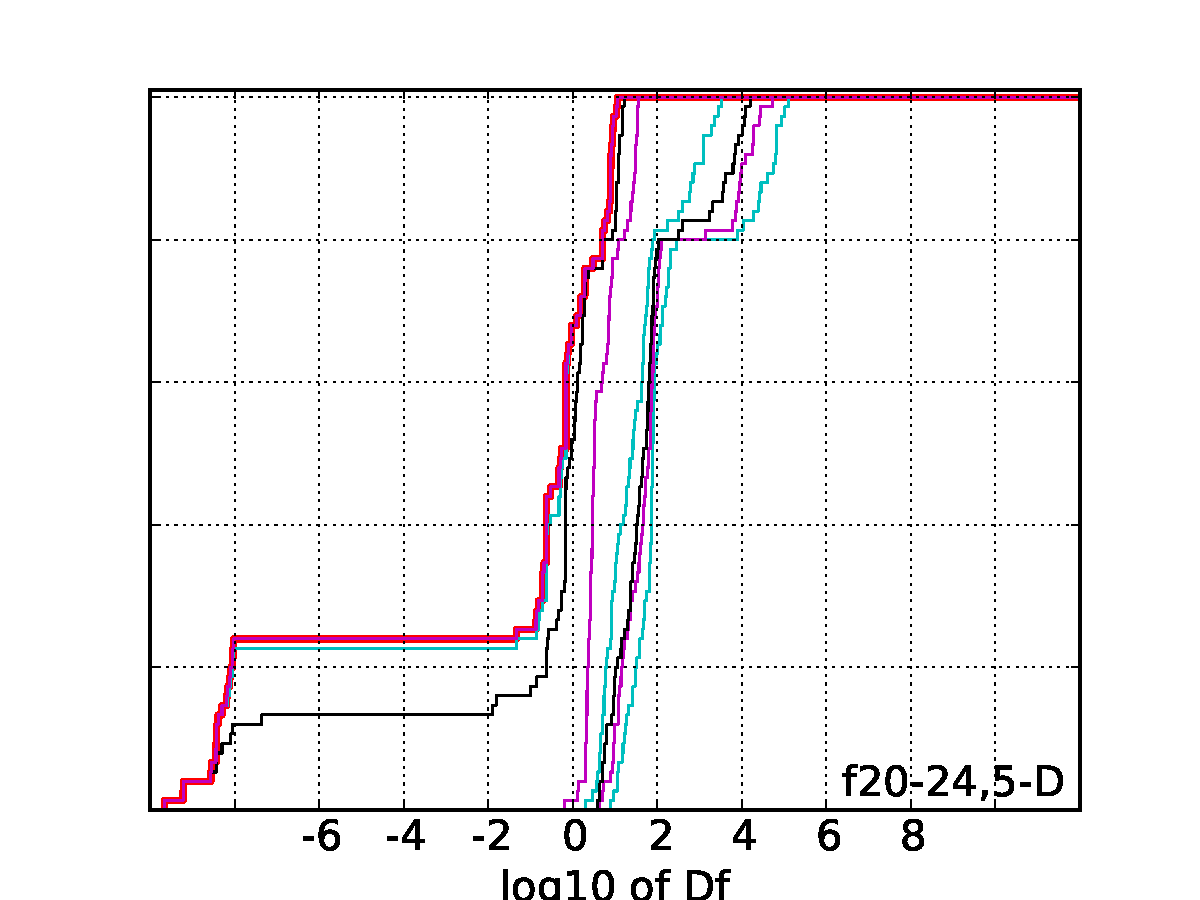
\includegraphics[width=0.2362\textwidth,trim=2.40cm 0 0 13mm, clip]{ppfvdistr_05D_mult2} &
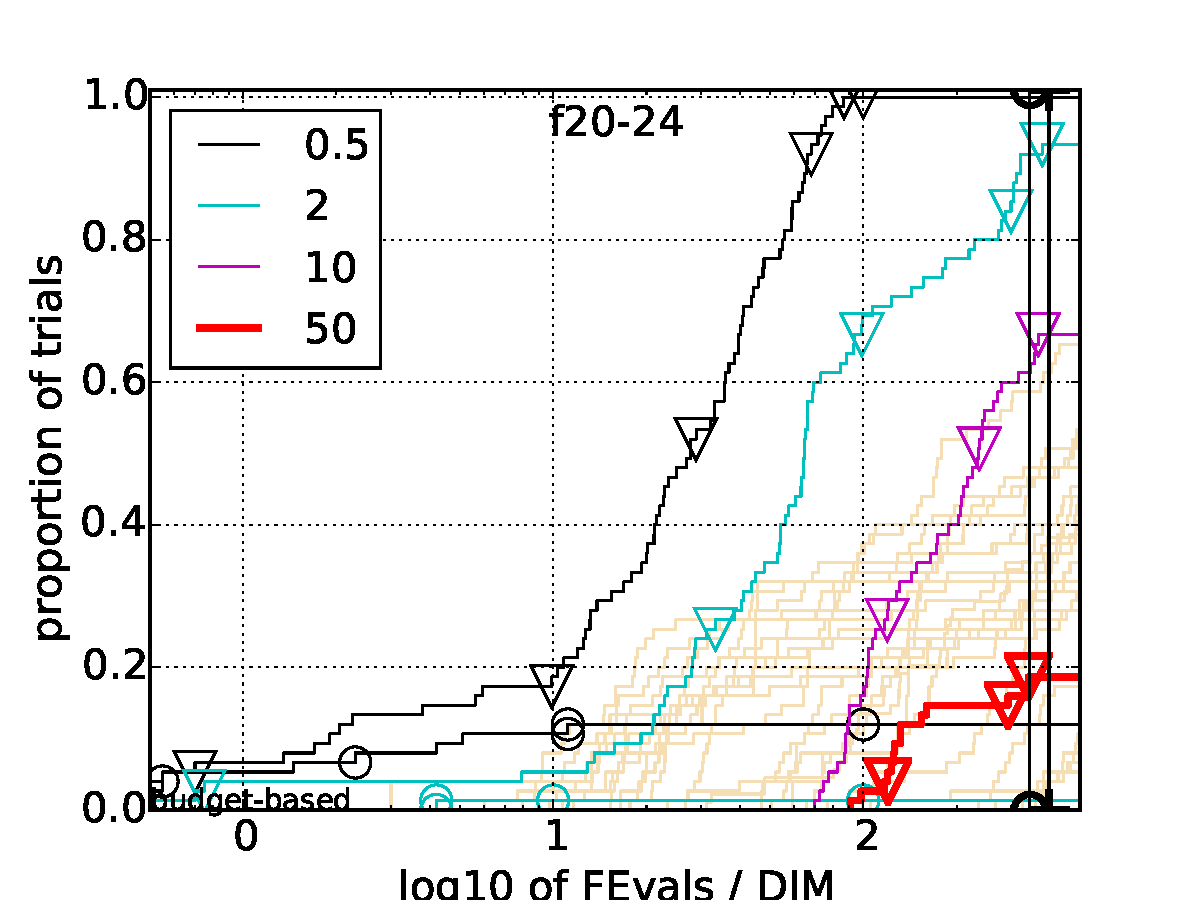
\includegraphics[width=0.268\textwidth,trim=0 0 0 13mm, clip]{pprldistr_20D_mult2} &
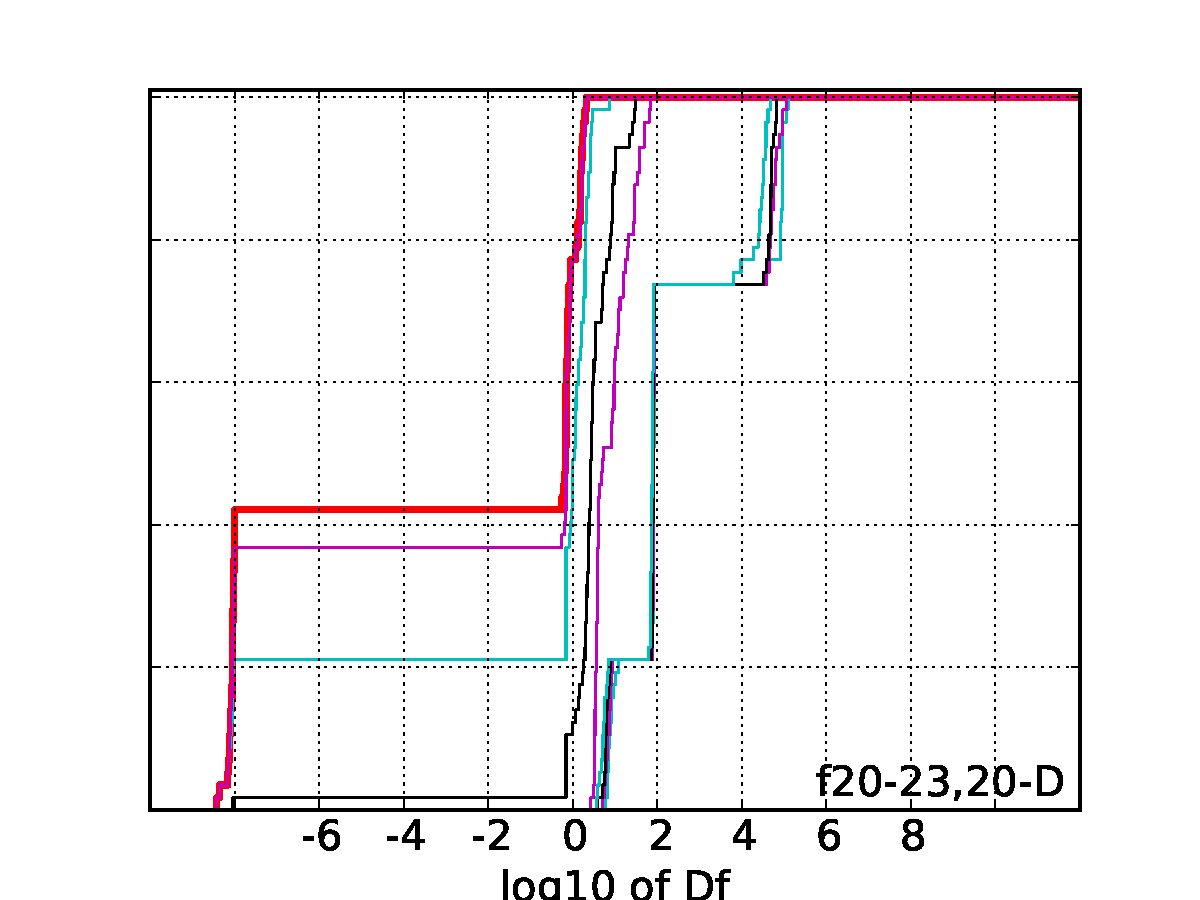
\includegraphics[width=0.2362\textwidth,trim=2.40cm 0 0 13mm, clip]{ppfvdistr_20D_mult2}\\[-2ex]
\rot{all functions}
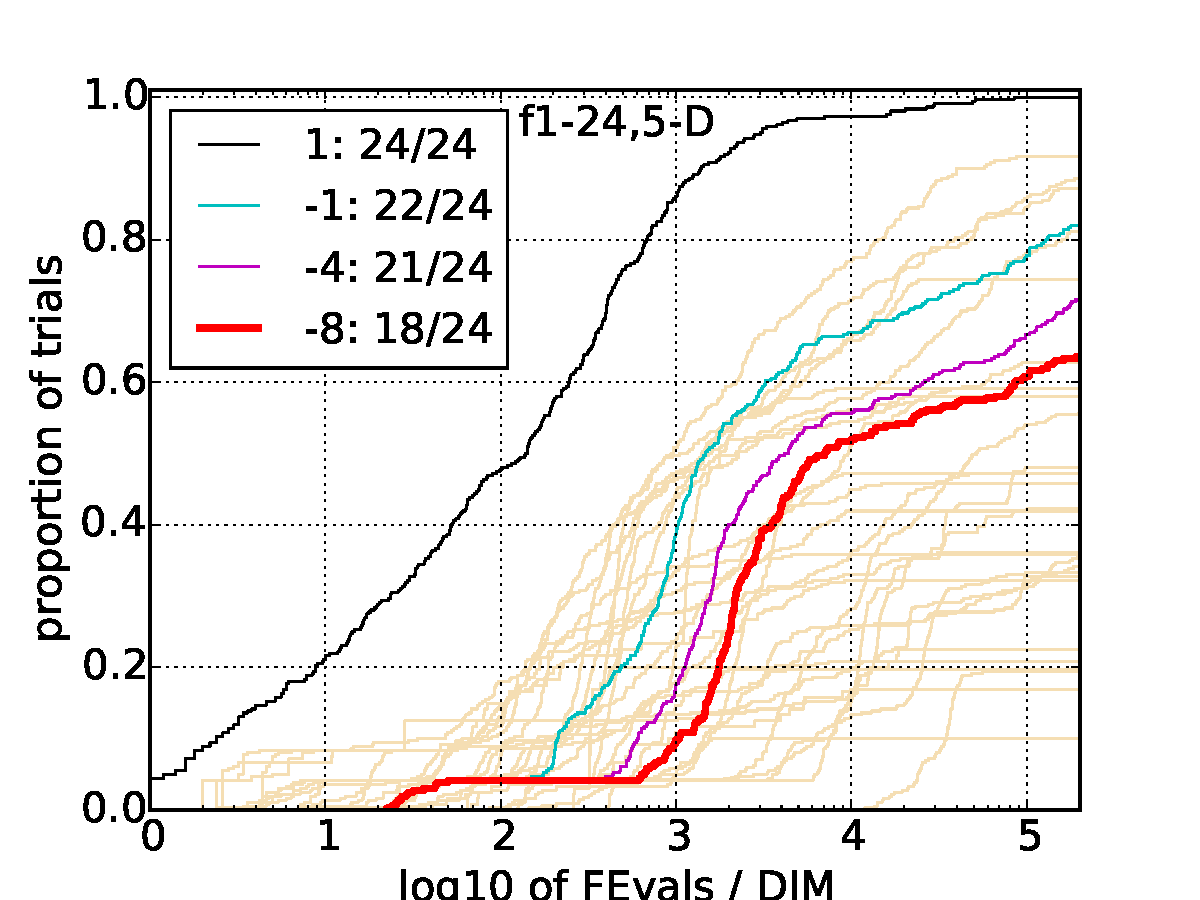
\includegraphics[width=0.268\textwidth,trim=0 0 0 13mm, clip]{pprldistr_05D_noiselessall} &
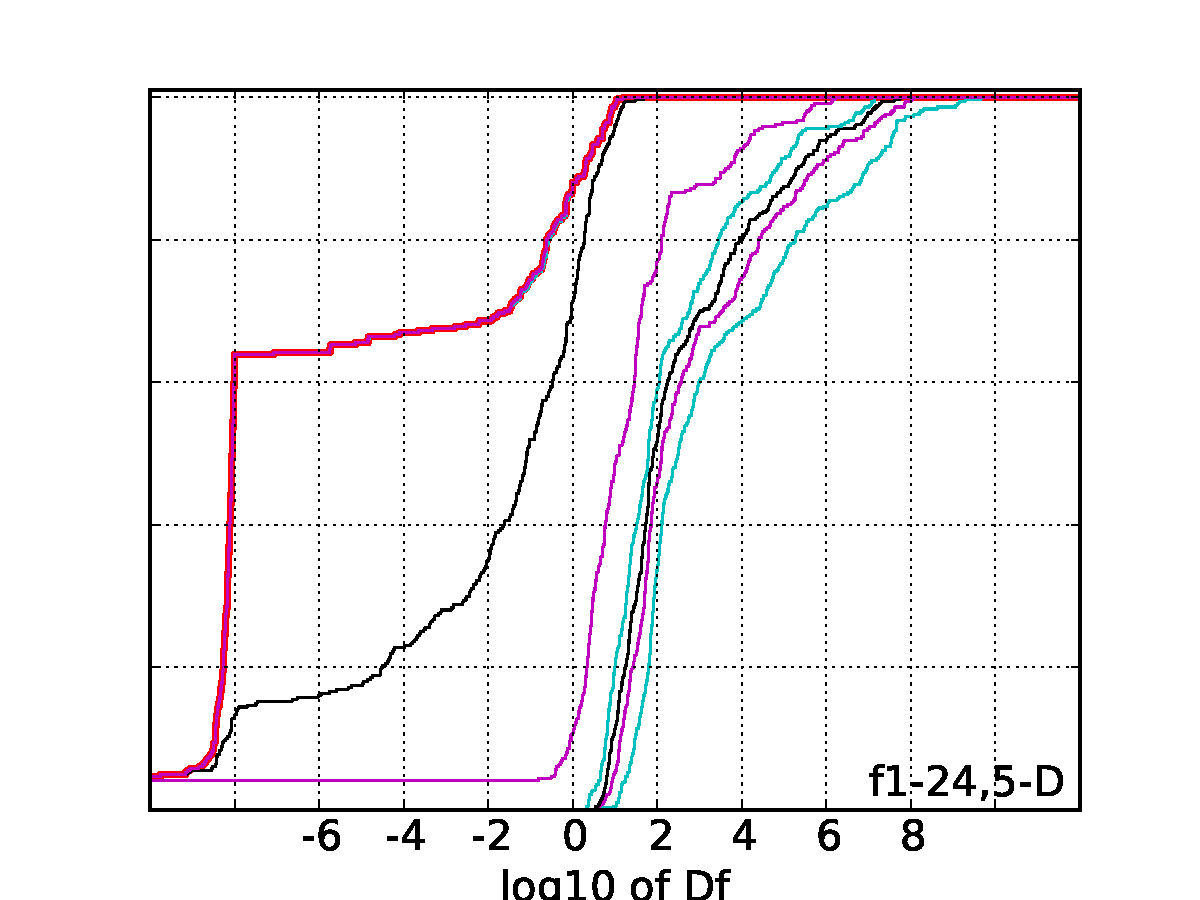
\includegraphics[width=0.2362\textwidth,trim=2.40cm 0 0 13mm, clip]{ppfvdistr_05D_noiselessall} &
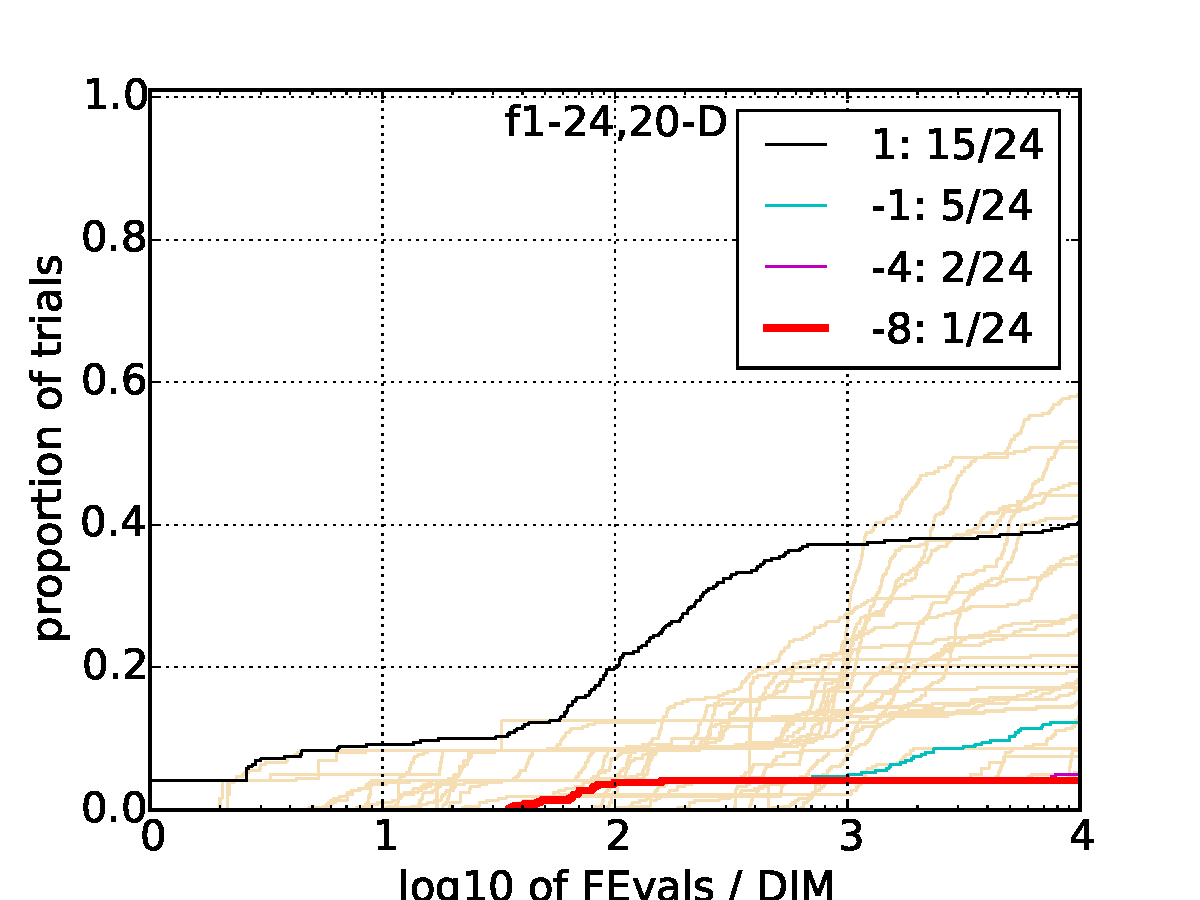
\includegraphics[width=0.268\textwidth,trim=0 0 0 13mm, clip]{pprldistr_20D_noiselessall} &
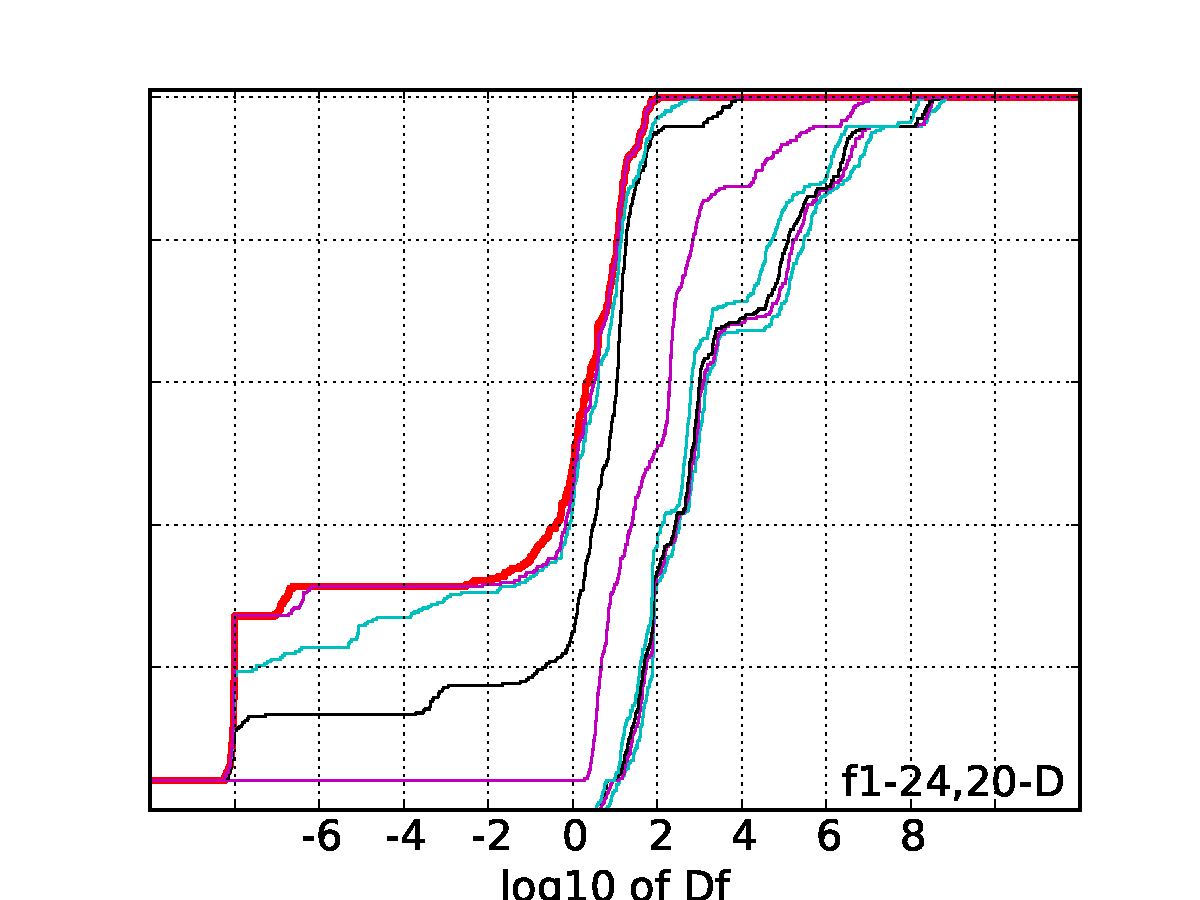
\includegraphics[width=0.2362\textwidth,trim=2.40cm 0 0 13mm, clip]{ppfvdistr_20D_noiselessall}
\vspace*{-0.5ex}
\end{tabular}
 \caption{\label{fig:RLDs}
 \bbobpprldistrlegend{}
 }
\end{figure*}
%%%%%%%%%%%%%%%%%%%%%%%%%%%%%%%%%%%%%%%%%%%%%%%%%%%%%%%%%%%%%%%%%%%%%%%%%%%%%%%


%%%%%%%%%%%%%%%%%%%%%%%%%%%%%%%%%%%%%%%%%%%%%%%%%%%%%%%%%%%%%%%%%%%%%%%%%%%%%%%
%%%%%%%%%%%%%%%%%%%%%%%%%%%%%%%%%%%%%%%%%%%%%%%%%%%%%%%%%%%%%%%%%%%%%%%%%%%%%%%

% ERT loss ratios (figure and table)

%%%%%%%%%%%%%%%%%%%%%%%%%%%%%%%%%%%%%%%%%%%%%%%%%%%%%%%%%%%%%%%%%%%%%%%%%%%%%%%
\begin{figure}
\centering
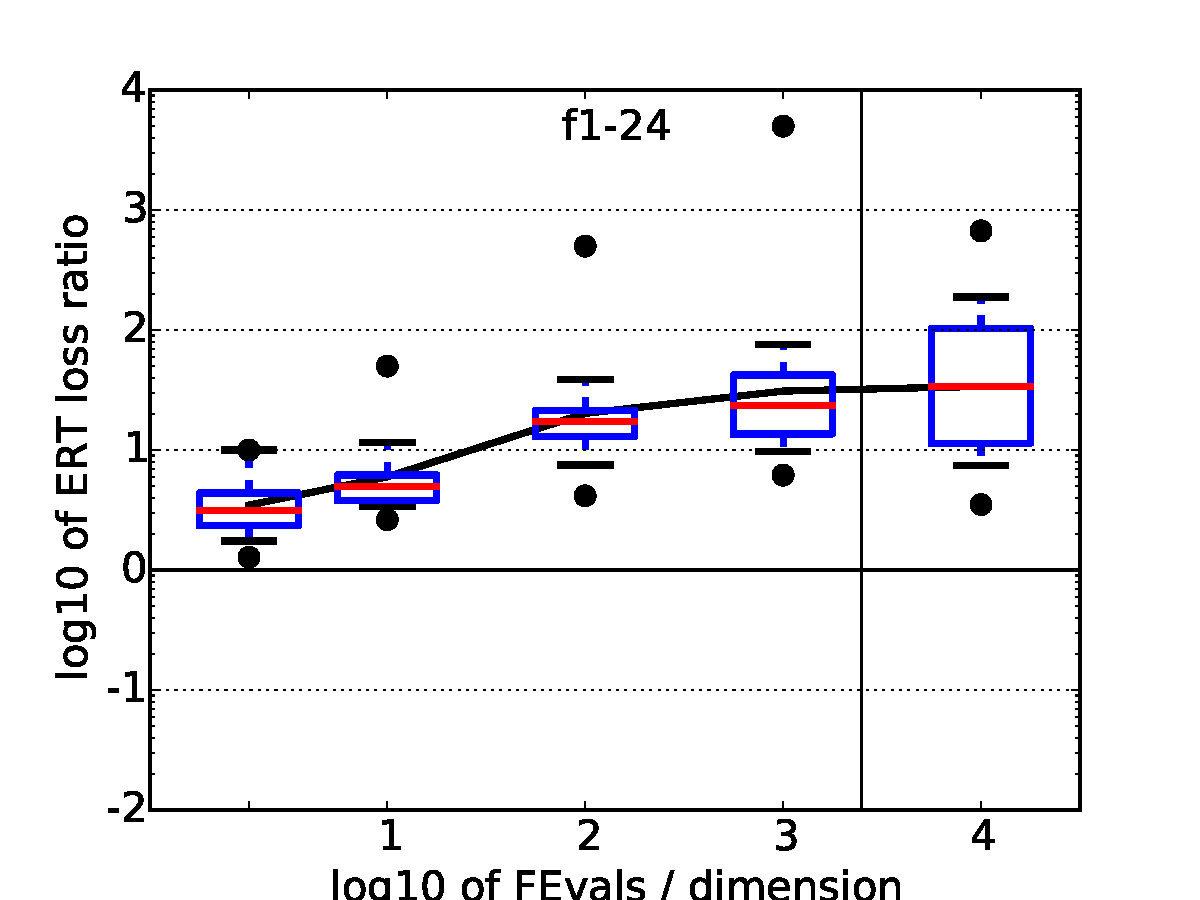
\includegraphics[width=0.24\textwidth,trim=0 0 16mm 12mm, clip]{pplogloss_05D_noiselessall}% 
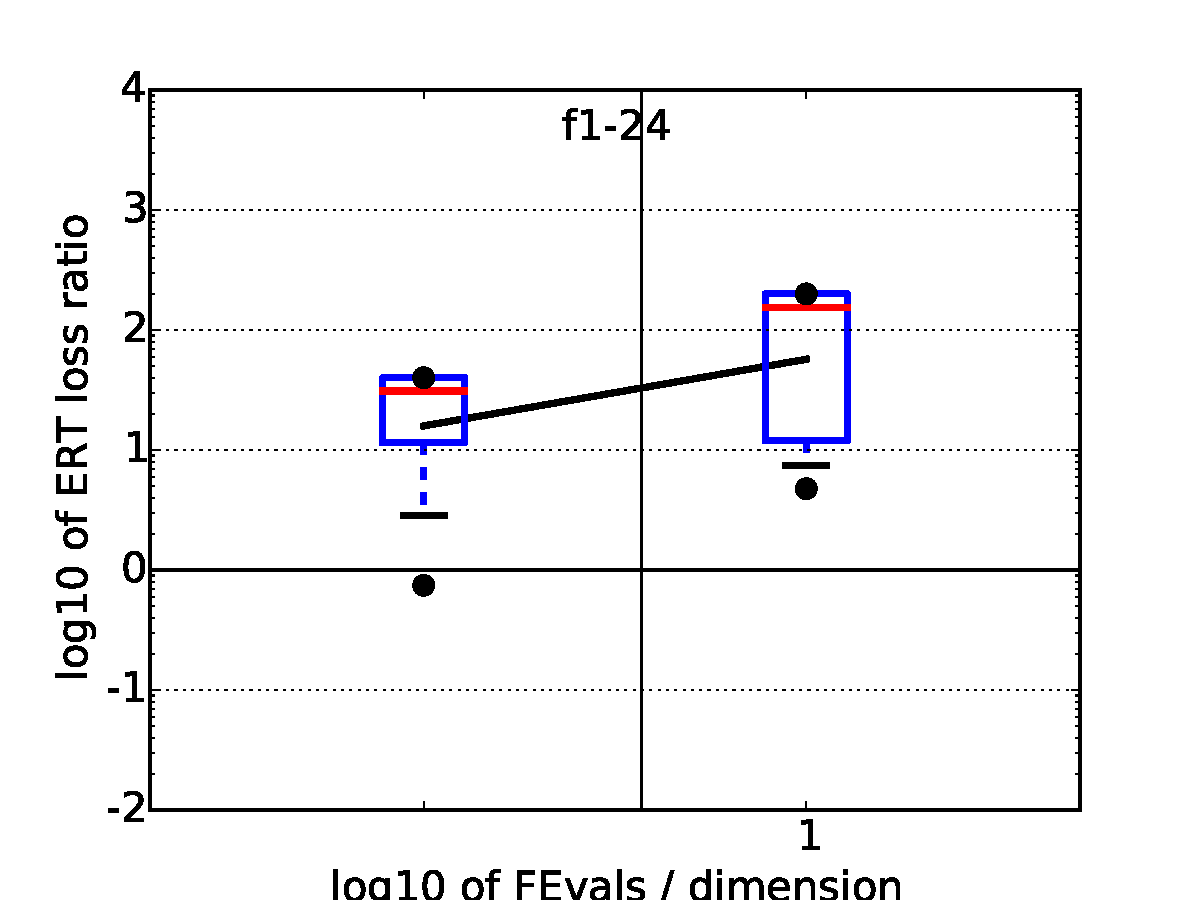
\includegraphics[width=0.24\textwidth,trim=7mm 0 9mm 12mm, clip]{pplogloss_20D_noiselessall}%
\\[-6.2ex]
\parbox{0.49\columnwidth}{\centering 5-D}%
\parbox{0.49\columnwidth}{\centering 20-D}\\[5ex]
%
\input{\bbobdatapath\algfolder pploglosstable_05D_noiselessall}\\
\input{\bbobdatapath\algfolder pploglosstable_20D_noiselessall}
\caption{\label{tab:ERTloss}%
\bbobloglosstablecaption{}
}
\end{figure}


%%%%%%%%%%%%%%%%%%%%%%%%%%%%%%%%%%%%%%%%%%%%%%%%%%%%%%%%%%%%%%%%%%%%%%%%%%%%%%%
%%%%%%%%%%%%%%%%%%%%%%%%%%%%%%%%%%%%%%%%%%%%%%%%%%%%%%%%%%%%%%%%%%%%%%%%%%%%%%%

% ERT loss ratios per function group

%%%%%%%%%%%%%%%%%%%%%%%%%%%%%%%%%%%%%%%%%%%%%%%%%%%%%%%%%%%%%%%%%%%%%%%%%%%%%%%
\begin{figure}
\begin{tabular}{@{}l@{}@{}l@{}}
\multicolumn{1}{c}{5-D} & \multicolumn{1}{c}{20-D}\\
%\rot{all functions}
%\hspace*{-2mm}
\rot{separable fcts}
\hspace*{-2mm}
\includegraphics[width=0.24\textwidth,trim=0 0 16mm 12mm, clip]{pplogloss_05D_separ} &
\includegraphics[width=0.24\textwidth,trim=7mm 0 9mm 12mm, clip]{pplogloss_20D_separ}\\[-2ex]
\rot[2]{moderate fcts}
\hspace*{-2mm}
\includegraphics[width=0.24\textwidth,trim=0 0 16mm 12mm, clip]{pplogloss_05D_lcond} &
\includegraphics[width=0.24\textwidth,trim=7mm 0 9mm 12mm, clip]{pplogloss_20D_lcond}\\[-2ex]
\rot[1.3]{ill-conditioned fcts}
\hspace*{-2mm}
\includegraphics[width=0.24\textwidth,trim=0 0 16mm 12mm, clip]{pplogloss_05D_hcond} &
\includegraphics[width=0.24\textwidth,trim=7mm 0 9mm 12mm, clip]{pplogloss_20D_hcond}\\[-2ex]
\rot[1.6]{multi-modal fcts}
\hspace*{-2mm}
\includegraphics[width=0.24\textwidth,trim=0 0 16mm 12mm, clip]{pplogloss_05D_multi} &
\includegraphics[width=0.24\textwidth,trim=7mm 0 9mm 12mm, clip]{pplogloss_20D_multi}\\[-2ex]
\rot[1.0]{weak structure fcts}
\hspace*{-2mm}
\includegraphics[width=0.24\textwidth,trim=0 0 16mm 12mm, clip]{pplogloss_05D_mult2} &
\includegraphics[width=0.24\textwidth,trim=7mm 0 9mm 12mm, clip]{pplogloss_20D_mult2}
\vspace*{-0.5ex}
\end{tabular}
 \caption{\label{fig:ERTlogloss}%
\bbobloglossfigurecaption{}
}
\end{figure}

%%%%%%%%%%%%%%%%%%%%%%%%%%%%%%%%%%%%%%%%%%%%%%%%%%%%%%%%%%%%%%%%%%%%%%%%%%%%%%%



%
% The following two commands are all you need in the
% initial runs of your .tex file to
% produce the bibliography for the citations in your paper.
\bibliographystyle{abbrv}
\bibliography{bbob}  % bbob.bib is the name of the Bibliography in this case
% You must have a proper ".bib" file
%  and remember to run:
% latex bibtex latex latex
% to resolve all references
% to create the ~.bbl file.  Insert that ~.bbl file into
% the .tex source file and comment out
% the command \texttt{{\char'134}thebibliography}.
%
% ACM needs 'a single self-contained file'!
%

\clearpage % otherwise the last figure might be missing
\end{document}
